% VIM: let g:vimtex_compiler_latexmk = { 'build_dir' : 'build', }


\documentclass{article} % For LaTeX2e
\usepackage{style/iclr,times}

% Optional math commands from https://github.com/goodfeli/dlbook_notation.
%%%%% NEW MATH DEFINITIONS %%%%%

\usepackage{amsmath,amsfonts,bm}

% Mark sections of captions for referring to divisions of figures
\newcommand{\figleft}{{\em (Left)}}
\newcommand{\figcenter}{{\em (Center)}}
\newcommand{\figright}{{\em (Right)}}
\newcommand{\figtop}{{\em (Top)}}
\newcommand{\figbottom}{{\em (Bottom)}}
\newcommand{\captiona}{{\em (a)}}
\newcommand{\captionb}{{\em (b)}}
\newcommand{\captionc}{{\em (c)}}
\newcommand{\captiond}{{\em (d)}}

% Highlight a newly defined term
\newcommand{\newterm}[1]{{\bf #1}}


% Figure reference, lower-case.
\def\figref#1{figure~\ref{#1}}
% Figure reference, capital. For start of sentence
\def\Figref#1{Figure~\ref{#1}}
\def\twofigref#1#2{figures \ref{#1} and \ref{#2}}
\def\quadfigref#1#2#3#4{figures \ref{#1}, \ref{#2}, \ref{#3} and \ref{#4}}
% Section reference, lower-case.
\def\secref#1{section~\ref{#1}}
% Section reference, capital.
\def\Secref#1{Section~\ref{#1}}
% Reference to two sections.
\def\twosecrefs#1#2{sections \ref{#1} and \ref{#2}}
% Reference to three sections.
\def\secrefs#1#2#3{sections \ref{#1}, \ref{#2} and \ref{#3}}
% Reference to an equation, lower-case.
\def\eqref#1{equation~\ref{#1}}
% Reference to an equation, upper case
\def\Eqref#1{Equation~\ref{#1}}
% A raw reference to an equation---avoid using if possible
\def\plaineqref#1{\ref{#1}}
% Reference to a chapter, lower-case.
\def\chapref#1{chapter~\ref{#1}}
% Reference to an equation, upper case.
\def\Chapref#1{Chapter~\ref{#1}}
% Reference to a range of chapters
\def\rangechapref#1#2{chapters\ref{#1}--\ref{#2}}
% Reference to an algorithm, lower-case.
\def\algref#1{algorithm~\ref{#1}}
% Reference to an algorithm, upper case.
\def\Algref#1{Algorithm~\ref{#1}}
\def\twoalgref#1#2{algorithms \ref{#1} and \ref{#2}}
\def\Twoalgref#1#2{Algorithms \ref{#1} and \ref{#2}}
% Reference to a part, lower case
\def\partref#1{part~\ref{#1}}
% Reference to a part, upper case
\def\Partref#1{Part~\ref{#1}}
\def\twopartref#1#2{parts \ref{#1} and \ref{#2}}

\def\ceil#1{\lceil #1 \rceil}
\def\floor#1{\lfloor #1 \rfloor}
\def\1{\bm{1}}
\newcommand{\train}{\mathcal{D}}
\newcommand{\valid}{\mathcal{D_{\mathrm{valid}}}}
\newcommand{\test}{\mathcal{D_{\mathrm{test}}}}

\def\eps{{\epsilon}}


% Random variables
\def\reta{{\textnormal{$\eta$}}}
\def\ra{{\textnormal{a}}}
\def\rb{{\textnormal{b}}}
\def\rc{{\textnormal{c}}}
\def\rd{{\textnormal{d}}}
\def\re{{\textnormal{e}}}
\def\rf{{\textnormal{f}}}
\def\rg{{\textnormal{g}}}
\def\rh{{\textnormal{h}}}
\def\ri{{\textnormal{i}}}
\def\rj{{\textnormal{j}}}
\def\rk{{\textnormal{k}}}
\def\rl{{\textnormal{l}}}
% rm is already a command, just don't name any random variables m
\def\rn{{\textnormal{n}}}
\def\ro{{\textnormal{o}}}
\def\rp{{\textnormal{p}}}
\def\rq{{\textnormal{q}}}
\def\rr{{\textnormal{r}}}
\def\rs{{\textnormal{s}}}
\def\rt{{\textnormal{t}}}
\def\ru{{\textnormal{u}}}
\def\rv{{\textnormal{v}}}
\def\rw{{\textnormal{w}}}
\def\rx{{\textnormal{x}}}
\def\ry{{\textnormal{y}}}
\def\rz{{\textnormal{z}}}

% Random vectors
\def\rvepsilon{{\mathbf{\epsilon}}}
\def\rvtheta{{\mathbf{\theta}}}
\def\rva{{\mathbf{a}}}
\def\rvb{{\mathbf{b}}}
\def\rvc{{\mathbf{c}}}
\def\rvd{{\mathbf{d}}}
\def\rve{{\mathbf{e}}}
\def\rvf{{\mathbf{f}}}
\def\rvg{{\mathbf{g}}}
\def\rvh{{\mathbf{h}}}
\def\rvu{{\mathbf{i}}}
\def\rvj{{\mathbf{j}}}
\def\rvk{{\mathbf{k}}}
\def\rvl{{\mathbf{l}}}
\def\rvm{{\mathbf{m}}}
\def\rvn{{\mathbf{n}}}
\def\rvo{{\mathbf{o}}}
\def\rvp{{\mathbf{p}}}
\def\rvq{{\mathbf{q}}}
\def\rvr{{\mathbf{r}}}
\def\rvs{{\mathbf{s}}}
\def\rvt{{\mathbf{t}}}
\def\rvu{{\mathbf{u}}}
\def\rvv{{\mathbf{v}}}
\def\rvw{{\mathbf{w}}}
\def\rvx{{\mathbf{x}}}
\def\rvy{{\mathbf{y}}}
\def\rvz{{\mathbf{z}}}

% Elements of random vectors
\def\erva{{\textnormal{a}}}
\def\ervb{{\textnormal{b}}}
\def\ervc{{\textnormal{c}}}
\def\ervd{{\textnormal{d}}}
\def\erve{{\textnormal{e}}}
\def\ervf{{\textnormal{f}}}
\def\ervg{{\textnormal{g}}}
\def\ervh{{\textnormal{h}}}
\def\ervi{{\textnormal{i}}}
\def\ervj{{\textnormal{j}}}
\def\ervk{{\textnormal{k}}}
\def\ervl{{\textnormal{l}}}
\def\ervm{{\textnormal{m}}}
\def\ervn{{\textnormal{n}}}
\def\ervo{{\textnormal{o}}}
\def\ervp{{\textnormal{p}}}
\def\ervq{{\textnormal{q}}}
\def\ervr{{\textnormal{r}}}
\def\ervs{{\textnormal{s}}}
\def\ervt{{\textnormal{t}}}
\def\ervu{{\textnormal{u}}}
\def\ervv{{\textnormal{v}}}
\def\ervw{{\textnormal{w}}}
\def\ervx{{\textnormal{x}}}
\def\ervy{{\textnormal{y}}}
\def\ervz{{\textnormal{z}}}

% Random matrices
\def\rmA{{\mathbf{A}}}
\def\rmB{{\mathbf{B}}}
\def\rmC{{\mathbf{C}}}
\def\rmD{{\mathbf{D}}}
\def\rmE{{\mathbf{E}}}
\def\rmF{{\mathbf{F}}}
\def\rmG{{\mathbf{G}}}
\def\rmH{{\mathbf{H}}}
\def\rmI{{\mathbf{I}}}
\def\rmJ{{\mathbf{J}}}
\def\rmK{{\mathbf{K}}}
\def\rmL{{\mathbf{L}}}
\def\rmM{{\mathbf{M}}}
\def\rmN{{\mathbf{N}}}
\def\rmO{{\mathbf{O}}}
\def\rmP{{\mathbf{P}}}
\def\rmQ{{\mathbf{Q}}}
\def\rmR{{\mathbf{R}}}
\def\rmS{{\mathbf{S}}}
\def\rmT{{\mathbf{T}}}
\def\rmU{{\mathbf{U}}}
\def\rmV{{\mathbf{V}}}
\def\rmW{{\mathbf{W}}}
\def\rmX{{\mathbf{X}}}
\def\rmY{{\mathbf{Y}}}
\def\rmZ{{\mathbf{Z}}}

% Elements of random matrices
\def\ermA{{\textnormal{A}}}
\def\ermB{{\textnormal{B}}}
\def\ermC{{\textnormal{C}}}
\def\ermD{{\textnormal{D}}}
\def\ermE{{\textnormal{E}}}
\def\ermF{{\textnormal{F}}}
\def\ermG{{\textnormal{G}}}
\def\ermH{{\textnormal{H}}}
\def\ermI{{\textnormal{I}}}
\def\ermJ{{\textnormal{J}}}
\def\ermK{{\textnormal{K}}}
\def\ermL{{\textnormal{L}}}
\def\ermM{{\textnormal{M}}}
\def\ermN{{\textnormal{N}}}
\def\ermO{{\textnormal{O}}}
\def\ermP{{\textnormal{P}}}
\def\ermQ{{\textnormal{Q}}}
\def\ermR{{\textnormal{R}}}
\def\ermS{{\textnormal{S}}}
\def\ermT{{\textnormal{T}}}
\def\ermU{{\textnormal{U}}}
\def\ermV{{\textnormal{V}}}
\def\ermW{{\textnormal{W}}}
\def\ermX{{\textnormal{X}}}
\def\ermY{{\textnormal{Y}}}
\def\ermZ{{\textnormal{Z}}}

% Vectors
\def\vzero{{\bm{0}}}
\def\vone{{\bm{1}}}
\def\vmu{{\bm{\mu}}}
\def\vtheta{{\bm{\theta}}}
\def\va{{\bm{a}}}
\def\vb{{\bm{b}}}
\def\vc{{\bm{c}}}
\def\vd{{\bm{d}}}
\def\ve{{\bm{e}}}
\def\vf{{\bm{f}}}
\def\vg{{\bm{g}}}
\def\vh{{\bm{h}}}
\def\vi{{\bm{i}}}
\def\vj{{\bm{j}}}
\def\vk{{\bm{k}}}
\def\vl{{\bm{l}}}
\def\vm{{\bm{m}}}
\def\vn{{\bm{n}}}
\def\vo{{\bm{o}}}
\def\vp{{\bm{p}}}
\def\vq{{\bm{q}}}
\def\vr{{\bm{r}}}
\def\vs{{\bm{s}}}
\def\vt{{\bm{t}}}
\def\vu{{\bm{u}}}
\def\vv{{\bm{v}}}
\def\vw{{\bm{w}}}
\def\vx{{\bm{x}}}
\def\vy{{\bm{y}}}
\def\vz{{\bm{z}}}

% Elements of vectors
\def\evalpha{{\alpha}}
\def\evbeta{{\beta}}
\def\evepsilon{{\epsilon}}
\def\evlambda{{\lambda}}
\def\evomega{{\omega}}
\def\evmu{{\mu}}
\def\evpsi{{\psi}}
\def\evsigma{{\sigma}}
\def\evtheta{{\theta}}
\def\eva{{a}}
\def\evb{{b}}
\def\evc{{c}}
\def\evd{{d}}
\def\eve{{e}}
\def\evf{{f}}
\def\evg{{g}}
\def\evh{{h}}
\def\evi{{i}}
\def\evj{{j}}
\def\evk{{k}}
\def\evl{{l}}
\def\evm{{m}}
\def\evn{{n}}
\def\evo{{o}}
\def\evp{{p}}
\def\evq{{q}}
\def\evr{{r}}
\def\evs{{s}}
\def\evt{{t}}
\def\evu{{u}}
\def\evv{{v}}
\def\evw{{w}}
\def\evx{{x}}
\def\evy{{y}}
\def\evz{{z}}

% Matrix
\def\mA{{\bm{A}}}
\def\mB{{\bm{B}}}
\def\mC{{\bm{C}}}
\def\mD{{\bm{D}}}
\def\mE{{\bm{E}}}
\def\mF{{\bm{F}}}
\def\mG{{\bm{G}}}
\def\mH{{\bm{H}}}
\def\mI{{\bm{I}}}
\def\mJ{{\bm{J}}}
\def\mK{{\bm{K}}}
\def\mL{{\bm{L}}}
\def\mM{{\bm{M}}}
\def\mN{{\bm{N}}}
\def\mO{{\bm{O}}}
\def\mP{{\bm{P}}}
\def\mQ{{\bm{Q}}}
\def\mR{{\bm{R}}}
\def\mS{{\bm{S}}}
\def\mT{{\bm{T}}}
\def\mU{{\bm{U}}}
\def\mV{{\bm{V}}}
\def\mW{{\bm{W}}}
\def\mX{{\bm{X}}}
\def\mY{{\bm{Y}}}
\def\mZ{{\bm{Z}}}
\def\mBeta{{\bm{\beta}}}
\def\mPhi{{\bm{\Phi}}}
\def\mLambda{{\bm{\Lambda}}}
\def\mSigma{{\bm{\Sigma}}}

% Tensor
\DeclareMathAlphabet{\mathsfit}{\encodingdefault}{\sfdefault}{m}{sl}
\SetMathAlphabet{\mathsfit}{bold}{\encodingdefault}{\sfdefault}{bx}{n}
\newcommand{\tens}[1]{\bm{\mathsfit{#1}}}
\def\tA{{\tens{A}}}
\def\tB{{\tens{B}}}
\def\tC{{\tens{C}}}
\def\tD{{\tens{D}}}
\def\tE{{\tens{E}}}
\def\tF{{\tens{F}}}
\def\tG{{\tens{G}}}
\def\tH{{\tens{H}}}
\def\tI{{\tens{I}}}
\def\tJ{{\tens{J}}}
\def\tK{{\tens{K}}}
\def\tL{{\tens{L}}}
\def\tM{{\tens{M}}}
\def\tN{{\tens{N}}}
\def\tO{{\tens{O}}}
\def\tP{{\tens{P}}}
\def\tQ{{\tens{Q}}}
\def\tR{{\tens{R}}}
\def\tS{{\tens{S}}}
\def\tT{{\tens{T}}}
\def\tU{{\tens{U}}}
\def\tV{{\tens{V}}}
\def\tW{{\tens{W}}}
\def\tX{{\tens{X}}}
\def\tY{{\tens{Y}}}
\def\tZ{{\tens{Z}}}


% Graph
\def\gA{{\mathcal{A}}}
\def\gB{{\mathcal{B}}}
\def\gC{{\mathcal{C}}}
\def\gD{{\mathcal{D}}}
\def\gE{{\mathcal{E}}}
\def\gF{{\mathcal{F}}}
\def\gG{{\mathcal{G}}}
\def\gH{{\mathcal{H}}}
\def\gI{{\mathcal{I}}}
\def\gJ{{\mathcal{J}}}
\def\gK{{\mathcal{K}}}
\def\gL{{\mathcal{L}}}
\def\gM{{\mathcal{M}}}
\def\gN{{\mathcal{N}}}
\def\gO{{\mathcal{O}}}
\def\gP{{\mathcal{P}}}
\def\gQ{{\mathcal{Q}}}
\def\gR{{\mathcal{R}}}
\def\gS{{\mathcal{S}}}
\def\gT{{\mathcal{T}}}
\def\gU{{\mathcal{U}}}
\def\gV{{\mathcal{V}}}
\def\gW{{\mathcal{W}}}
\def\gX{{\mathcal{X}}}
\def\gY{{\mathcal{Y}}}
\def\gZ{{\mathcal{Z}}}

% Sets
\def\sA{{\mathbb{A}}}
\def\sB{{\mathbb{B}}}
\def\sC{{\mathbb{C}}}
\def\sD{{\mathbb{D}}}
% Don't use a set called E, because this would be the same as our symbol
% for expectation.
\def\sF{{\mathbb{F}}}
\def\sG{{\mathbb{G}}}
\def\sH{{\mathbb{H}}}
\def\sI{{\mathbb{I}}}
\def\sJ{{\mathbb{J}}}
\def\sK{{\mathbb{K}}}
\def\sL{{\mathbb{L}}}
\def\sM{{\mathbb{M}}}
\def\sN{{\mathbb{N}}}
\def\sO{{\mathbb{O}}}
\def\sP{{\mathbb{P}}}
\def\sQ{{\mathbb{Q}}}
\def\sR{{\mathbb{R}}}
\def\sS{{\mathbb{S}}}
\def\sT{{\mathbb{T}}}
\def\sU{{\mathbb{U}}}
\def\sV{{\mathbb{V}}}
\def\sW{{\mathbb{W}}}
\def\sX{{\mathbb{X}}}
\def\sY{{\mathbb{Y}}}
\def\sZ{{\mathbb{Z}}}

% Entries of a matrix
\def\emLambda{{\Lambda}}
\def\emA{{A}}
\def\emB{{B}}
\def\emC{{C}}
\def\emD{{D}}
\def\emE{{E}}
\def\emF{{F}}
\def\emG{{G}}
\def\emH{{H}}
\def\emI{{I}}
\def\emJ{{J}}
\def\emK{{K}}
\def\emL{{L}}
\def\emM{{M}}
\def\emN{{N}}
\def\emO{{O}}
\def\emP{{P}}
\def\emQ{{Q}}
\def\emR{{R}}
\def\emS{{S}}
\def\emT{{T}}
\def\emU{{U}}
\def\emV{{V}}
\def\emW{{W}}
\def\emX{{X}}
\def\emY{{Y}}
\def\emZ{{Z}}
\def\emSigma{{\Sigma}}

% entries of a tensor
% Same font as tensor, without \bm wrapper
\newcommand{\etens}[1]{\mathsfit{#1}}
\def\etLambda{{\etens{\Lambda}}}
\def\etA{{\etens{A}}}
\def\etB{{\etens{B}}}
\def\etC{{\etens{C}}}
\def\etD{{\etens{D}}}
\def\etE{{\etens{E}}}
\def\etF{{\etens{F}}}
\def\etG{{\etens{G}}}
\def\etH{{\etens{H}}}
\def\etI{{\etens{I}}}
\def\etJ{{\etens{J}}}
\def\etK{{\etens{K}}}
\def\etL{{\etens{L}}}
\def\etM{{\etens{M}}}
\def\etN{{\etens{N}}}
\def\etO{{\etens{O}}}
\def\etP{{\etens{P}}}
\def\etQ{{\etens{Q}}}
\def\etR{{\etens{R}}}
\def\etS{{\etens{S}}}
\def\etT{{\etens{T}}}
\def\etU{{\etens{U}}}
\def\etV{{\etens{V}}}
\def\etW{{\etens{W}}}
\def\etX{{\etens{X}}}
\def\etY{{\etens{Y}}}
\def\etZ{{\etens{Z}}}

% The true underlying data generating distribution
\newcommand{\pdata}{p_{\rm{data}}}
% The empirical distribution defined by the training set
\newcommand{\ptrain}{\hat{p}_{\rm{data}}}
\newcommand{\Ptrain}{\hat{P}_{\rm{data}}}
% The model distribution
\newcommand{\pmodel}{p_{\rm{model}}}
\newcommand{\Pmodel}{P_{\rm{model}}}
\newcommand{\ptildemodel}{\tilde{p}_{\rm{model}}}
% Stochastic autoencoder distributions
\newcommand{\pencode}{p_{\rm{encoder}}}
\newcommand{\pdecode}{p_{\rm{decoder}}}
\newcommand{\precons}{p_{\rm{reconstruct}}}

\newcommand{\laplace}{\mathrm{Laplace}} % Laplace distribution

\newcommand{\E}{\mathbb{E}}
\newcommand{\Ls}{\mathcal{L}}
\newcommand{\R}{\mathbb{R}}
\newcommand{\emp}{\tilde{p}}
\newcommand{\lr}{\alpha}
\newcommand{\reg}{\lambda}
\newcommand{\rect}{\mathrm{rectifier}}
\newcommand{\softmax}{\mathrm{softmax}}
\newcommand{\sigmoid}{\sigma}
\newcommand{\softplus}{\zeta}
\newcommand{\KL}{D_{\mathrm{KL}}}
\newcommand{\Var}{\mathrm{Var}}
\newcommand{\standarderror}{\mathrm{SE}}
\newcommand{\Cov}{\mathrm{Cov}}
% Wolfram Mathworld says $L^2$ is for function spaces and $\ell^2$ is for vectors
% But then they seem to use $L^2$ for vectors throughout the site, and so does
% wikipedia.
\newcommand{\normlzero}{L^0}
\newcommand{\normlone}{L^1}
\newcommand{\normltwo}{L^2}
\newcommand{\normlp}{L^p}
\newcommand{\normmax}{L^\infty}

\newcommand{\parents}{Pa} % See usage in notation.tex. Chosen to match Daphne's book.

\DeclareMathOperator*{\argmax}{arg\,max}
\DeclareMathOperator*{\argmin}{arg\,min}

\DeclareMathOperator{\sign}{sign}
\DeclareMathOperator{\Tr}{Tr}
\let\ab\allowbreak


\usepackage{hyperref}
\usepackage{url}
\usepackage{tikz}
\usepackage{subcaption}
\usepackage{mathtools}

\newcommand{\leftsib}{{ls}}
\newcommand{\rightsib}{{lr}}
\newcommand{\leftcol}{{lc}}
\newcommand{\rightcol}{{rc}}
\newcommand{\children}{{c}}
\newcommand{\parent}{{p}}
\newcommand{\hpred}{{\vh^{\star}}}

\title{Modeling Structured Data with Relational Decomposition}

% Authors must not appear in the submitted version. They should be hidden
% as long as the \iclrfinalcopy macro remains commented out below.
% Non-anonymous submissions will be rejected without review.

\author{Antiquus S.~Hippocampus, Natalia Cerebro \& Amelie P. Amygdale \thanks{ Use footnote for providing further information
about author (webpage, alternative address)---\emph{not} for acknowledging
funding agencies.  Funding acknowledgements go at the end of the paper.} \\
Department of Computer Science\\
Cranberry-Lemon University\\
Pittsburgh, PA 15213, USA \\
\texttt{\{hippo,brain,jen\}@cs.cranberry-lemon.edu} \\
\And
Ji Q. Ren \& Yevgeny LeNet \\
Department of Computational Neuroscience \\
University of the Witwatersrand \\
Joburg, South Africa \\
\texttt{\{robot,net\}@wits.ac.za} \\
\AND
Coauthor \\
Affiliation \\
Address \\
\texttt{email}
}

% The \author macro works with any number of authors. There are two commands
% used to separate the names and addresses of multiple authors: \And and \AND.
%
% Using \And between authors leaves it to \LaTeX{} to determine where to break
% the lines. Using \AND forces a linebreak at that point. So, if \LaTeX{}
% puts 3 of 4 authors names on the first line, and the last on the second
% line, try using \AND instead of \And before the third author name.

\newcommand{\fix}{\marginpar{FIX}}
\newcommand{\new}{\marginpar{NEW}}

\hypersetup{
  colorlinks   = true, %Colours links instead of ugly boxes
  urlcolor     = blue, %Colour for external hyperlinks
  linkcolor    = blue, %Colour of internal links
	citecolor   = blue %Colour of citations
}


%\iclrfinalcopy % Uncomment for camera-ready version, but NOT for submission.
\begin{document}


\maketitle

\begin{abstract}
\end{abstract}

%Unrolling a graph to a tree, equivalent to message passing. Identifying loops.
%DRNN paper claims TreeLSTM can't be used for decoding. Sure it can.

%More general recursive neural networks and structures that work beyond RNNs are  
%rarer. Seq2Tree, Tree2Seq, Tree2Tree, Graphs
%Trees reduce "long-term"ness (and functional decomposition)

%Only pass in a bottom-up encoding?

% Generating graphs with cycles/message-passing?

%Variable misuse, assuming all variables exist and don't need to be declared.

%Semantic encoding -> syntactic decoding
		
%Decoding can use progressively less information.

%Encoding and decoding can even go in different directions

%Try to have an enncoding that doesn't contain any other bugs.

%Encoding:  all the leaves have different outputs. Hmmm...

%The encoder basically becomes the decoder if trained to just predict `next''
%token generatively. If not, we need to pass all possible nodes to the decoder 
%as ``starting points''.

%If two nodes share the same decomposition, then the model can't distinguish 
%them.

%We move topology prediction to be before the node generation?

%for (int i = 0; i < 10; i++) {
%	printf("%d\n", i);
%}

\section{Introduction}\label{sec:introduction}

Traditionally, tasks in program analysis treated source code as a linear 
sequence of tokens.  Without any further modeling, a recurrent neural network 
(RNN) trained on such sequences is theoretically able to learn the underlying 
dependencies---the \textit{structure}---of the sequence elements.  The structure 
is implicit in the parameters of the RNN and in the values of the hidden states.
\begin{figure}[ht]
\begin{center}
	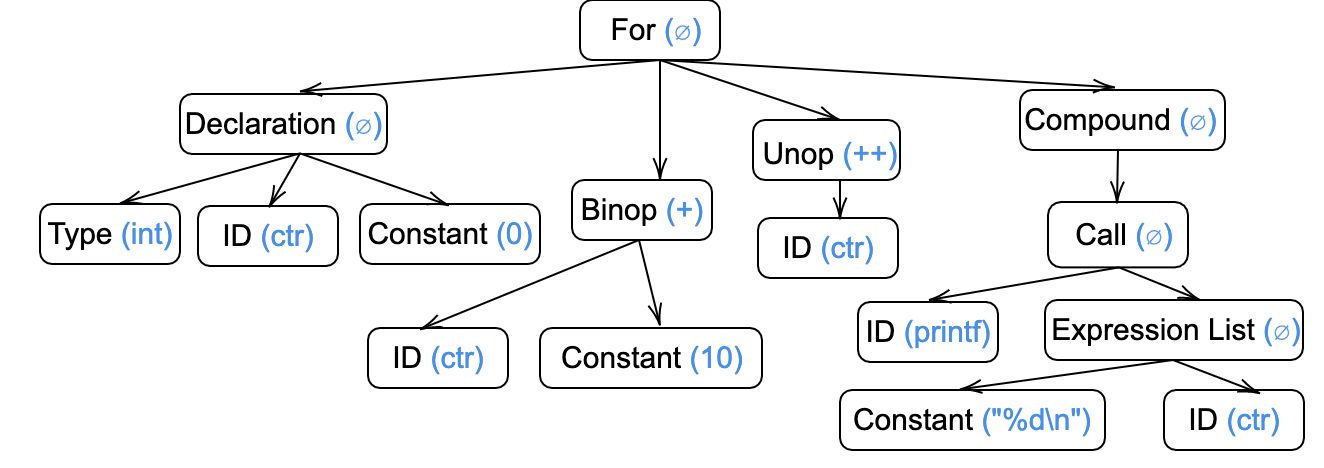
\includegraphics[width=\textwidth]{figures/ast.png}
\end{center}
\caption{An example abstract syntax tree for the C programming 
language.}\label{fig:ast}
\end{figure}



However, while source code may be linear, its execution is fundamentally 
nonlinear. A sequential model trained on source code has to learn these 
nonlinearities, often without any actual sense of a language's semantics.  A 
program's abstract syntax tree (AST), as seen in Figure~\ref{fig:ast}, is one 
step closer to modeling the nonlinearity in a program. Recent work has placed 
increasing emphasis on \textit{explicitly} modeling the underlying structure of 
such nonlinear data (see Section~\ref{sec:related}).


%By explicitly working on parse trees for natural language tasks and abstract 
%syntax trees (ASTs) for program analysis tasks, we simplify the learning task
%Even BERT, though linear, removes the directionality bias inherenet in RNNs.  
%What benefits?  Nonlinearity.  Limits on the ability for the RNN to memorize


To this end, we introduce the notion of \textit{relational decomposition}, with 
which one can readily express complicated dependencies between elements in 
structured data. At a high level, relational decomposition involves applying 
prior knowledge to break down structured data into smaller chunks that are 
individually easier to learn, and then aggregating the results from all chunks. 

For example, if we know in advance that a particular node in a tree only depends 
on its immediate ancestors, then we can narrow the focus of the learning task to 
just that relational path through the tree. In decomposing a problem, we find 
that being able to use relational operators directly is invaluable, such as 
using composition to specify ``siblings of my parent''. Given these operators, 
we find that many mechanisms such as attention are readily expressed in 
relational terms, even without applying relational decomposition.



%Relational decomposition provides a natural way of modeling trees as 
%combinations of relationships. For example, doubly-recurrent neural networks 
%(DRNNs)\cite{alvarez2016tree} decompose nodes into parent paths and 
%left-sibling paths (see Figure~\ref{fig:broken}).
%In the case of DRNNs, the relative paths form sequences that can be trained with 
%two independent RNNs. However, an individual relation may be modeled with 
%feed-forward neural network, bidirectional RNNs, graph neural networks, or even 
%a non-deep-learning module.

%A further challenge in modeling source code is arbitrary identifiers. In 
%section, we demonstrate how relational decomposition over ASTs simplifies this 
%task.
%
%Although we use ASTs as motivating examples throughout the paper, relational 
%decomposition readily applies to other structured tasks. 


%Applications of machine learning to programming offer great promise: bug 
%detection, automatic program repair, program synthesis, code understanding, 
%autocompletion, variable name suggestion, program translation, program 
%analysis, automated test generation, and so on.  However, two properties of 
%source code present recurring difficulty to modern algorithms: arbitrary 
%user-defined identifiers and nonlinearity.  Arbitrary identifiers mean that two 
%variables with the same purpose may not share a name, and also neural networks 
%have a finite dictionary. We return to the point of arbitrary identifiers later 
%in the paper, for now focusing on nonlinearity.


% int ctr = 0;
% for (int i = 0; i < 10; i++)
% for (int j = 0; j < 10; j++)
% for (int k = 0; k < 10; k++)
% ctr += 1; return 10;

%" These results suggest that it is the
%need to integrate structures far apart in the sentence that characterizes the tasks where recursive
%models surpass recurrent models."
% \cite{DBLP:journals/corr/LiJH15}
% Also, outputs are much more likely to compile/be syntactically valid

%In recent years, increasing effort has focused on using the inherent structure 
%of source code.  In doing so, we can improve training speed and learnability.  
%However, In general, this requires learning the relationship between 
%\textit{all} variables in the input and output.  Attempt to model the structure 
%directly.  Inductive bias
%
%The simplest example of a structure is a sequence, for which RNNs (and LSTMs) 
%have thrived.  They have transformed speech recognition, language translation, 
%etc.

\begin{figure}[ht]\label{fig:preorder}
\begin{center}


\tikzset{every picture/.style={line width=0.75pt}} %set default line width to 0.75pt        

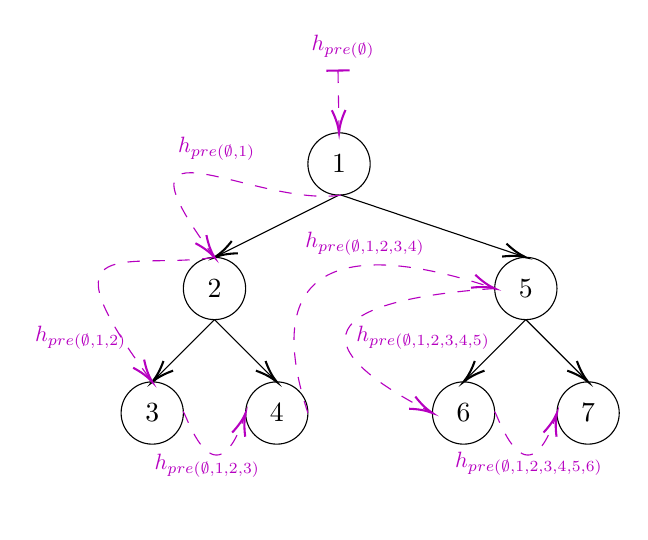
\begin{tikzpicture}[x=0.75pt,y=0.75pt,yscale=-1,xscale=1]
%uncomment if require: \path (0,247.3125); %set diagram left start at 0, and has height of 247.3125

%Shape: Circle [id:dp5747539528933221] 
\draw   (150,75) .. controls (150,66.72) and (156.72,60) .. (165,60) .. controls (173.28,60) and (180,66.72) .. (180,75) .. controls (180,83.28) and (173.28,90) .. (165,90) .. controls (156.72,90) and (150,83.28) .. (150,75) -- cycle ;
%Shape: Circle [id:dp6584741963271383] 
\draw   (90,135) .. controls (90,126.72) and (96.72,120) .. (105,120) .. controls (113.28,120) and (120,126.72) .. (120,135) .. controls (120,143.28) and (113.28,150) .. (105,150) .. controls (96.72,150) and (90,143.28) .. (90,135) -- cycle ;
%Shape: Circle [id:dp42608384351679063] 
\draw   (240,135) .. controls (240,126.72) and (246.72,120) .. (255,120) .. controls (263.28,120) and (270,126.72) .. (270,135) .. controls (270,143.28) and (263.28,150) .. (255,150) .. controls (246.72,150) and (240,143.28) .. (240,135) -- cycle ;
%Shape: Circle [id:dp4039562507165959] 
\draw   (60,195) .. controls (60,186.72) and (66.72,180) .. (75,180) .. controls (83.28,180) and (90,186.72) .. (90,195) .. controls (90,203.28) and (83.28,210) .. (75,210) .. controls (66.72,210) and (60,203.28) .. (60,195) -- cycle ;
%Shape: Circle [id:dp6061665496522999] 
\draw   (120,195) .. controls (120,186.72) and (126.72,180) .. (135,180) .. controls (143.28,180) and (150,186.72) .. (150,195) .. controls (150,203.28) and (143.28,210) .. (135,210) .. controls (126.72,210) and (120,203.28) .. (120,195) -- cycle ;
%Straight Lines [id:da040054788995673274] 
\draw    (165,90) -- (106.79,119.11) ;
\draw [shift={(105,120)}, rotate = 333.43] [color={rgb, 255:red, 0; green, 0; blue, 0 }  ][line width=0.75]    (10.93,-3.29) .. controls (6.95,-1.4) and (3.31,-0.3) .. (0,0) .. controls (3.31,0.3) and (6.95,1.4) .. (10.93,3.29)   ;

%Straight Lines [id:da9417356343431731] 
\draw    (166,90) -- (253.1,119.36) ;
\draw [shift={(255,120)}, rotate = 198.63] [color={rgb, 255:red, 0; green, 0; blue, 0 }  ][line width=0.75]    (10.93,-3.29) .. controls (6.95,-1.4) and (3.31,-0.3) .. (0,0) .. controls (3.31,0.3) and (6.95,1.4) .. (10.93,3.29)   ;

%Straight Lines [id:da7471003825026084] 
\draw    (105,150) -- (76.41,178.59) ;
\draw [shift={(75,180)}, rotate = 315] [color={rgb, 255:red, 0; green, 0; blue, 0 }  ][line width=0.75]    (10.93,-3.29) .. controls (6.95,-1.4) and (3.31,-0.3) .. (0,0) .. controls (3.31,0.3) and (6.95,1.4) .. (10.93,3.29)   ;

%Straight Lines [id:da3919517743443004] 
\draw    (105,150) -- (133.59,178.59) ;
\draw [shift={(135,180)}, rotate = 225] [color={rgb, 255:red, 0; green, 0; blue, 0 }  ][line width=0.75]    (10.93,-3.29) .. controls (6.95,-1.4) and (3.31,-0.3) .. (0,0) .. controls (3.31,0.3) and (6.95,1.4) .. (10.93,3.29)   ;

%Shape: Circle [id:dp09204588637656741] 
\draw   (210,195) .. controls (210,186.72) and (216.72,180) .. (225,180) .. controls (233.28,180) and (240,186.72) .. (240,195) .. controls (240,203.28) and (233.28,210) .. (225,210) .. controls (216.72,210) and (210,203.28) .. (210,195) -- cycle ;
%Shape: Circle [id:dp4405799901518632] 
\draw   (270,195) .. controls (270,186.72) and (276.72,180) .. (285,180) .. controls (293.28,180) and (300,186.72) .. (300,195) .. controls (300,203.28) and (293.28,210) .. (285,210) .. controls (276.72,210) and (270,203.28) .. (270,195) -- cycle ;
%Straight Lines [id:da9350681939269714] 
\draw    (255,150) -- (226.41,178.59) ;
\draw [shift={(225,180)}, rotate = 315] [color={rgb, 255:red, 0; green, 0; blue, 0 }  ][line width=0.75]    (10.93,-3.29) .. controls (6.95,-1.4) and (3.31,-0.3) .. (0,0) .. controls (3.31,0.3) and (6.95,1.4) .. (10.93,3.29)   ;

%Straight Lines [id:da6947341181570368] 
\draw    (255,150) -- (283.59,178.59) ;
\draw [shift={(285,180)}, rotate = 225] [color={rgb, 255:red, 0; green, 0; blue, 0 }  ][line width=0.75]    (10.93,-3.29) .. controls (6.95,-1.4) and (3.31,-0.3) .. (0,0) .. controls (3.31,0.3) and (6.95,1.4) .. (10.93,3.29)   ;

%Curve Lines [id:da39887266209810046] 
\draw [color={rgb, 255:red, 182; green, 0; blue, 192 }  ,draw opacity=1 ] [dash pattern={on 4.5pt off 4.5pt}]  (166,90) .. controls (124.21,96.28) and (50.74,46.81) .. (104.18,118.9) ;
\draw [shift={(105,120)}, rotate = 233.26] [color={rgb, 255:red, 182; green, 0; blue, 192 }  ,draw opacity=1 ][line width=0.75]    (10.93,-3.29) .. controls (6.95,-1.4) and (3.31,-0.3) .. (0,0) .. controls (3.31,0.3) and (6.95,1.4) .. (10.93,3.29)   ;

%Curve Lines [id:da20716783829208452] 
\draw [color={rgb, 255:red, 182; green, 0; blue, 192 }  ,draw opacity=1 ] [dash pattern={on 4.5pt off 4.5pt}]  (105,120) .. controls (63.21,126.28) and (20.43,106.51) .. (74.18,178.9) ;
\draw [shift={(75,180)}, rotate = 233.26] [color={rgb, 255:red, 182; green, 0; blue, 192 }  ,draw opacity=1 ][line width=0.75]    (10.93,-3.29) .. controls (6.95,-1.4) and (3.31,-0.3) .. (0,0) .. controls (3.31,0.3) and (6.95,1.4) .. (10.93,3.29)   ;

%Curve Lines [id:da03343755971007978] 
\draw [color={rgb, 255:red, 182; green, 0; blue, 192 }  ,draw opacity=1 ] [dash pattern={on 4.5pt off 4.5pt}]  (150,195) .. controls (124.63,117.7) and (174.99,113.35) .. (239.03,134.68) ;
\draw [shift={(240,135)}, rotate = 198.57999999999998] [color={rgb, 255:red, 182; green, 0; blue, 192 }  ,draw opacity=1 ][line width=0.75]    (10.93,-3.29) .. controls (6.95,-1.4) and (3.31,-0.3) .. (0,0) .. controls (3.31,0.3) and (6.95,1.4) .. (10.93,3.29)   ;

%Curve Lines [id:da25925997339396334] 
\draw [color={rgb, 255:red, 182; green, 0; blue, 192 }  ,draw opacity=1 ] [dash pattern={on 4.5pt off 4.5pt}]  (240,135) .. controls (177.81,139.29) and (130.97,154.16) .. (208.82,194.39) ;
\draw [shift={(210,195)}, rotate = 207.1] [color={rgb, 255:red, 182; green, 0; blue, 192 }  ,draw opacity=1 ][line width=0.75]    (10.93,-3.29) .. controls (6.95,-1.4) and (3.31,-0.3) .. (0,0) .. controls (3.31,0.3) and (6.95,1.4) .. (10.93,3.29)   ;

%Curve Lines [id:da04019975701917122] 
\draw [color={rgb, 255:red, 182; green, 0; blue, 192 }  ,draw opacity=1 ] [dash pattern={on 4.5pt off 4.5pt}]  (240,195) .. controls (239.51,189.37) and (254.2,242.24) .. (269.54,196.42) ;
\draw [shift={(270,195)}, rotate = 467.79] [color={rgb, 255:red, 182; green, 0; blue, 192 }  ,draw opacity=1 ][line width=0.75]    (10.93,-3.29) .. controls (6.95,-1.4) and (3.31,-0.3) .. (0,0) .. controls (3.31,0.3) and (6.95,1.4) .. (10.93,3.29)   ;

%Straight Lines [id:da47300784385513417] 
\draw [color={rgb, 255:red, 182; green, 0; blue, 192 }  ,draw opacity=1 ] [dash pattern={on 4.5pt off 4.5pt}]  (164.5,30) -- (164.97,58) ;
\draw [shift={(165,60)}, rotate = 269.05] [color={rgb, 255:red, 182; green, 0; blue, 192 }  ,draw opacity=1 ][line width=0.75]    (10.93,-3.29) .. controls (6.95,-1.4) and (3.31,-0.3) .. (0,0) .. controls (3.31,0.3) and (6.95,1.4) .. (10.93,3.29)   ;
\draw [shift={(164.5,30)}, rotate = 269.05] [color={rgb, 255:red, 182; green, 0; blue, 192 }  ,draw opacity=1 ][line width=0.75]    (0,5.59) -- (0,-5.59)   ;
%Curve Lines [id:da4854965313512276] 
\draw [color={rgb, 255:red, 182; green, 0; blue, 192 }  ,draw opacity=1 ] [dash pattern={on 4.5pt off 4.5pt}]  (90,195) .. controls (89.51,189.37) and (104.2,242.24) .. (119.54,196.42) ;
\draw [shift={(120,195)}, rotate = 467.79] [color={rgb, 255:red, 182; green, 0; blue, 192 }  ,draw opacity=1 ][line width=0.75]    (10.93,-3.29) .. controls (6.95,-1.4) and (3.31,-0.3) .. (0,0) .. controls (3.31,0.3) and (6.95,1.4) .. (10.93,3.29)   ;


% Text Node
\draw (165,75) node  [align=left] {1};
% Text Node
\draw (105,135) node  [align=left] {2};
% Text Node
\draw (255,135) node  [align=left] {5};
% Text Node
\draw (120,138) node  [align=left] {$ $};
% Text Node
\draw (75,195) node  [align=left] {3};
% Text Node
\draw (135,195) node  [align=left] {4};
% Text Node
\draw (225,195) node  [align=left] {6};
% Text Node
\draw (285,195) node  [align=left] {7};
% Text Node
\draw (167,18.5) node [scale=0.8,color={rgb, 255:red, 182; green, 0; blue, 192 }  ,opacity=1 ] [align=left] {$\displaystyle h_{pre( \emptyset )}$};
% Text Node
\draw (106,67.5) node [scale=0.8,color={rgb, 255:red, 182; green, 0; blue, 192 }  ,opacity=1 ] [align=left] {$\displaystyle h_{pre( \emptyset ,1)}$};
% Text Node
\draw (40.5,158.5) node [scale=0.8,color={rgb, 255:red, 182; green, 0; blue, 192 }  ,opacity=1 ] [align=left] {$\displaystyle h_{pre( \emptyset ,1,2)}$};
% Text Node
\draw (101.5,220.5) node [scale=0.8,color={rgb, 255:red, 182; green, 0; blue, 192 }  ,opacity=1 ] [align=left] {$\displaystyle h_{pre( \emptyset ,1,2,3)}$};
% Text Node
\draw (177.5,113.5) node [scale=0.8,color={rgb, 255:red, 182; green, 0; blue, 192 }  ,opacity=1 ] [align=left] {$\displaystyle h_{pre( \emptyset ,1,2,3,4)}$};
% Text Node
\draw (205.5,158.5) node [scale=0.8,color={rgb, 255:red, 182; green, 0; blue, 192 }  ,opacity=1 ] [align=left] {$\displaystyle h_{pre( \emptyset ,1,2,3,4,5)}$};
% Text Node
\draw (256.5,219.5) node [scale=0.8,color={rgb, 255:red, 182; green, 0; blue, 192 }  ,opacity=1 ] [align=left] {$\displaystyle h_{pre( \emptyset ,1,2,3,4,5,6)}$};


\end{tikzpicture}

\end{center}
\caption{Preorder}
\end{figure}

\begin{figure}[ht]\label{fig:left_subtree}
\begin{center}


\tikzset{every picture/.style={line width=0.75pt}} %set default line width to 0.75pt        

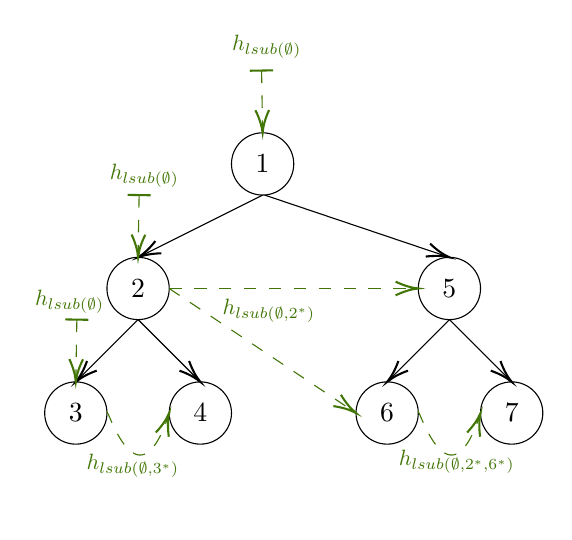
\begin{tikzpicture}[x=0.75pt,y=0.75pt,yscale=-1,xscale=1]
%uncomment if require: \path (0,247.3125); %set diagram left start at 0, and has height of 247.3125

%Shape: Circle [id:dp6157879539497779] 
\draw   (150,75) .. controls (150,66.72) and (156.72,60) .. (165,60) .. controls (173.28,60) and (180,66.72) .. (180,75) .. controls (180,83.28) and (173.28,90) .. (165,90) .. controls (156.72,90) and (150,83.28) .. (150,75) -- cycle ;
%Shape: Circle [id:dp6839112001955174] 
\draw   (90,135) .. controls (90,126.72) and (96.72,120) .. (105,120) .. controls (113.28,120) and (120,126.72) .. (120,135) .. controls (120,143.28) and (113.28,150) .. (105,150) .. controls (96.72,150) and (90,143.28) .. (90,135) -- cycle ;
%Shape: Circle [id:dp18336869601957861] 
\draw   (240,135) .. controls (240,126.72) and (246.72,120) .. (255,120) .. controls (263.28,120) and (270,126.72) .. (270,135) .. controls (270,143.28) and (263.28,150) .. (255,150) .. controls (246.72,150) and (240,143.28) .. (240,135) -- cycle ;
%Shape: Circle [id:dp9914306980420791] 
\draw   (60,195) .. controls (60,186.72) and (66.72,180) .. (75,180) .. controls (83.28,180) and (90,186.72) .. (90,195) .. controls (90,203.28) and (83.28,210) .. (75,210) .. controls (66.72,210) and (60,203.28) .. (60,195) -- cycle ;
%Shape: Circle [id:dp45458813355193795] 
\draw   (120,195) .. controls (120,186.72) and (126.72,180) .. (135,180) .. controls (143.28,180) and (150,186.72) .. (150,195) .. controls (150,203.28) and (143.28,210) .. (135,210) .. controls (126.72,210) and (120,203.28) .. (120,195) -- cycle ;
%Straight Lines [id:da6107312542319738] 
\draw    (165,90) -- (106.79,119.11) ;
\draw [shift={(105,120)}, rotate = 333.43] [color={rgb, 255:red, 0; green, 0; blue, 0 }  ][line width=0.75]    (10.93,-3.29) .. controls (6.95,-1.4) and (3.31,-0.3) .. (0,0) .. controls (3.31,0.3) and (6.95,1.4) .. (10.93,3.29)   ;

%Straight Lines [id:da9010042020513775] 
\draw    (166,90) -- (253.1,119.36) ;
\draw [shift={(255,120)}, rotate = 198.63] [color={rgb, 255:red, 0; green, 0; blue, 0 }  ][line width=0.75]    (10.93,-3.29) .. controls (6.95,-1.4) and (3.31,-0.3) .. (0,0) .. controls (3.31,0.3) and (6.95,1.4) .. (10.93,3.29)   ;

%Straight Lines [id:da28436007454589474] 
\draw    (105,150) -- (76.41,178.59) ;
\draw [shift={(75,180)}, rotate = 315] [color={rgb, 255:red, 0; green, 0; blue, 0 }  ][line width=0.75]    (10.93,-3.29) .. controls (6.95,-1.4) and (3.31,-0.3) .. (0,0) .. controls (3.31,0.3) and (6.95,1.4) .. (10.93,3.29)   ;

%Straight Lines [id:da35477685401761994] 
\draw    (105,150) -- (133.59,178.59) ;
\draw [shift={(135,180)}, rotate = 225] [color={rgb, 255:red, 0; green, 0; blue, 0 }  ][line width=0.75]    (10.93,-3.29) .. controls (6.95,-1.4) and (3.31,-0.3) .. (0,0) .. controls (3.31,0.3) and (6.95,1.4) .. (10.93,3.29)   ;

%Shape: Circle [id:dp08089268518255177] 
\draw   (210,195) .. controls (210,186.72) and (216.72,180) .. (225,180) .. controls (233.28,180) and (240,186.72) .. (240,195) .. controls (240,203.28) and (233.28,210) .. (225,210) .. controls (216.72,210) and (210,203.28) .. (210,195) -- cycle ;
%Shape: Circle [id:dp31235408856004776] 
\draw   (270,195) .. controls (270,186.72) and (276.72,180) .. (285,180) .. controls (293.28,180) and (300,186.72) .. (300,195) .. controls (300,203.28) and (293.28,210) .. (285,210) .. controls (276.72,210) and (270,203.28) .. (270,195) -- cycle ;
%Straight Lines [id:da13902395629734543] 
\draw    (255,150) -- (226.41,178.59) ;
\draw [shift={(225,180)}, rotate = 315] [color={rgb, 255:red, 0; green, 0; blue, 0 }  ][line width=0.75]    (10.93,-3.29) .. controls (6.95,-1.4) and (3.31,-0.3) .. (0,0) .. controls (3.31,0.3) and (6.95,1.4) .. (10.93,3.29)   ;

%Straight Lines [id:da6903149917947036] 
\draw    (255,150) -- (283.59,178.59) ;
\draw [shift={(285,180)}, rotate = 225] [color={rgb, 255:red, 0; green, 0; blue, 0 }  ][line width=0.75]    (10.93,-3.29) .. controls (6.95,-1.4) and (3.31,-0.3) .. (0,0) .. controls (3.31,0.3) and (6.95,1.4) .. (10.93,3.29)   ;

%Straight Lines [id:da5391406594009582] 
\draw [color={rgb, 255:red, 65; green, 117; blue, 5 }  ,draw opacity=1 ] [dash pattern={on 4.5pt off 4.5pt}]  (164.5,30) -- (164.97,58) ;
\draw [shift={(165,60)}, rotate = 269.05] [color={rgb, 255:red, 65; green, 117; blue, 5 }  ,draw opacity=1 ][line width=0.75]    (10.93,-3.29) .. controls (6.95,-1.4) and (3.31,-0.3) .. (0,0) .. controls (3.31,0.3) and (6.95,1.4) .. (10.93,3.29)   ;
\draw [shift={(164.5,30)}, rotate = 269.05] [color={rgb, 255:red, 65; green, 117; blue, 5 }  ,draw opacity=1 ][line width=0.75]    (0,5.59) -- (0,-5.59)   ;
%Straight Lines [id:da22601358599192456] 
\draw [color={rgb, 255:red, 65; green, 117; blue, 5 }  ,draw opacity=1 ] [dash pattern={on 4.5pt off 4.5pt}]  (105.5,90) -- (105.03,118) ;
\draw [shift={(105,120)}, rotate = 270.95] [color={rgb, 255:red, 65; green, 117; blue, 5 }  ,draw opacity=1 ][line width=0.75]    (10.93,-3.29) .. controls (6.95,-1.4) and (3.31,-0.3) .. (0,0) .. controls (3.31,0.3) and (6.95,1.4) .. (10.93,3.29)   ;
\draw [shift={(105.5,90)}, rotate = 270.95] [color={rgb, 255:red, 65; green, 117; blue, 5 }  ,draw opacity=1 ][line width=0.75]    (0,5.59) -- (0,-5.59)   ;
%Straight Lines [id:da6509181719744728] 
\draw [color={rgb, 255:red, 65; green, 117; blue, 5 }  ,draw opacity=1 ] [dash pattern={on 4.5pt off 4.5pt}]  (75.5,150) -- (75.03,178) ;
\draw [shift={(75,180)}, rotate = 270.95] [color={rgb, 255:red, 65; green, 117; blue, 5 }  ,draw opacity=1 ][line width=0.75]    (10.93,-3.29) .. controls (6.95,-1.4) and (3.31,-0.3) .. (0,0) .. controls (3.31,0.3) and (6.95,1.4) .. (10.93,3.29)   ;
\draw [shift={(75.5,150)}, rotate = 270.95] [color={rgb, 255:red, 65; green, 117; blue, 5 }  ,draw opacity=1 ][line width=0.75]    (0,5.59) -- (0,-5.59)   ;
%Straight Lines [id:da25480615087237357] 
\draw [color={rgb, 255:red, 65; green, 117; blue, 5 }  ,draw opacity=1 ] [dash pattern={on 4.5pt off 4.5pt}]  (120,135) -- (238,135) ;
\draw [shift={(240,135)}, rotate = 180] [color={rgb, 255:red, 65; green, 117; blue, 5 }  ,draw opacity=1 ][line width=0.75]    (10.93,-3.29) .. controls (6.95,-1.4) and (3.31,-0.3) .. (0,0) .. controls (3.31,0.3) and (6.95,1.4) .. (10.93,3.29)   ;

%Straight Lines [id:da5158226852684309] 
\draw [color={rgb, 255:red, 65; green, 117; blue, 5 }  ,draw opacity=1 ] [dash pattern={on 4.5pt off 4.5pt}]  (120,135) -- (208.34,193.89) ;
\draw [shift={(210,195)}, rotate = 213.69] [color={rgb, 255:red, 65; green, 117; blue, 5 }  ,draw opacity=1 ][line width=0.75]    (10.93,-3.29) .. controls (6.95,-1.4) and (3.31,-0.3) .. (0,0) .. controls (3.31,0.3) and (6.95,1.4) .. (10.93,3.29)   ;

%Curve Lines [id:da39446511277388496] 
\draw [color={rgb, 255:red, 65; green, 117; blue, 5 }  ,draw opacity=1 ] [dash pattern={on 4.5pt off 4.5pt}]  (90,195) .. controls (89.51,189.37) and (104.2,242.24) .. (119.54,196.42) ;
\draw [shift={(120,195)}, rotate = 467.79] [color={rgb, 255:red, 65; green, 117; blue, 5 }  ,draw opacity=1 ][line width=0.75]    (10.93,-3.29) .. controls (6.95,-1.4) and (3.31,-0.3) .. (0,0) .. controls (3.31,0.3) and (6.95,1.4) .. (10.93,3.29)   ;

%Curve Lines [id:da7449295923622143] 
\draw [color={rgb, 255:red, 65; green, 117; blue, 5 }  ,draw opacity=1 ] [dash pattern={on 4.5pt off 4.5pt}]  (240,195) .. controls (239.51,189.37) and (254.2,242.24) .. (269.54,196.42) ;
\draw [shift={(270,195)}, rotate = 467.79] [color={rgb, 255:red, 65; green, 117; blue, 5 }  ,draw opacity=1 ][line width=0.75]    (10.93,-3.29) .. controls (6.95,-1.4) and (3.31,-0.3) .. (0,0) .. controls (3.31,0.3) and (6.95,1.4) .. (10.93,3.29)   ;


% Text Node
\draw (165,75) node  [align=left] {1};
% Text Node
\draw (105,135) node  [align=left] {2};
% Text Node
\draw (255,135) node  [align=left] {5};
% Text Node
\draw (120,138) node  [align=left] {$ $};
% Text Node
\draw (75,195) node  [align=left] {3};
% Text Node
\draw (135,195) node  [align=left] {4};
% Text Node
\draw (225,195) node  [align=left] {6};
% Text Node
\draw (285,195) node  [align=left] {7};
% Text Node
\draw (167,18.5) node [scale=0.8,color={rgb, 255:red, 65; green, 117; blue, 5 }  ,opacity=1 ] [align=left] {$\displaystyle h_{lsub( \emptyset )}$};
% Text Node
\draw (108,80.5) node [scale=0.8,color={rgb, 255:red, 65; green, 117; blue, 5 }  ,opacity=1 ] [align=left] {$\displaystyle h_{lsub( \emptyset )}$};
% Text Node
\draw (102.5,220.5) node [scale=0.8,color={rgb, 255:red, 65; green, 117; blue, 5 }  ,opacity=1 ] [align=left] {$\displaystyle h_{lsub\left( \emptyset ,3^{*}\right)}$};
% Text Node
\draw (72,141.5) node [scale=0.8,color={rgb, 255:red, 65; green, 117; blue, 5 }  ,opacity=1 ] [align=left] {$\displaystyle h_{lsub( \emptyset )}$};
% Text Node
\draw (168,145.5) node [scale=0.8,color={rgb, 255:red, 65; green, 117; blue, 5 }  ,opacity=1 ] [align=left] {$\displaystyle h_{lsub\left( \emptyset ,2^{*}\right)}$};
% Text Node
\draw (258.5,218.5) node [scale=0.8,color={rgb, 255:red, 65; green, 117; blue, 5 }  ,opacity=1 ] [align=left] {$\displaystyle h_{lsub\left( \emptyset ,2^{*} ,6^{*}\right)}$};


\end{tikzpicture}

\end{center}
\caption{Left subtree}
\end{figure}

\begin{figure}[ht]\label{fig:cell}
\begin{center}



\tikzset{every picture/.style={line width=0.75pt}} %set default line width to 0.75pt        

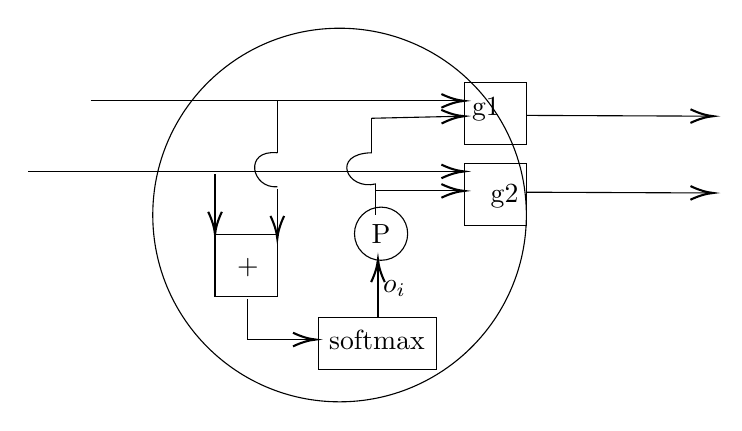
\begin{tikzpicture}[x=0.75pt,y=0.75pt,yscale=-1,xscale=1]
%uncomment if require: \path (0,247.3125); %set diagram left start at 0, and has height of 247.3125

%Shape: Circle [id:dp6083722186206264] 
\draw   (300,90) .. controls (300,40.29) and (340.29,0) .. (390,0) .. controls (439.71,0) and (480,40.29) .. (480,90) .. controls (480,139.71) and (439.71,180) .. (390,180) .. controls (340.29,180) and (300,139.71) .. (300,90) -- cycle ;
%Straight Lines [id:da561245922461306] 
\draw    (270,35) -- (448,35) ;
\draw [shift={(450,35)}, rotate = 180] [color={rgb, 255:red, 0; green, 0; blue, 0 }  ][line width=0.75]    (10.93,-3.29) .. controls (6.95,-1.4) and (3.31,-0.3) .. (0,0) .. controls (3.31,0.3) and (6.95,1.4) .. (10.93,3.29)   ;

%Straight Lines [id:da18790606634377727] 
\draw    (240,69) -- (448,69) ;
\draw [shift={(450,69)}, rotate = 180] [color={rgb, 255:red, 0; green, 0; blue, 0 }  ][line width=0.75]    (10.93,-3.29) .. controls (6.95,-1.4) and (3.31,-0.3) .. (0,0) .. controls (3.31,0.3) and (6.95,1.4) .. (10.93,3.29)   ;

%Shape: Square [id:dp2745914981980191] 
\draw   (450,26) -- (480,26) -- (480,56) -- (450,56) -- cycle ;
%Shape: Square [id:dp4400376186234609] 
\draw   (450,65) -- (480,65) -- (480,95) -- (450,95) -- cycle ;
%Shape: Square [id:dp5494449586600998] 
\draw   (330,99.38) -- (360,99.38) -- (360,129.38) -- (330,129.38) -- cycle ;
%Straight Lines [id:da5818908117859822] 
\draw    (345.5,150) -- (376.5,150) ;
\draw [shift={(378.5,150)}, rotate = 180] [color={rgb, 255:red, 0; green, 0; blue, 0 }  ][line width=0.75]    (10.93,-3.29) .. controls (6.95,-1.4) and (3.31,-0.3) .. (0,0) .. controls (3.31,0.3) and (6.95,1.4) .. (10.93,3.29)   ;

%Shape: Rectangle [id:dp8507803775022897] 
\draw   (380,139.38) -- (436.5,139.38) -- (436.5,164.38) -- (380,164.38) -- cycle ;
%Straight Lines [id:da5079909504409219] 
\draw    (408.5,139.38) -- (408.5,113.38) ;
\draw [shift={(408.5,111.38)}, rotate = 450] [color={rgb, 255:red, 0; green, 0; blue, 0 }  ][line width=0.75]    (10.93,-3.29) .. controls (6.95,-1.4) and (3.31,-0.3) .. (0,0) .. controls (3.31,0.3) and (6.95,1.4) .. (10.93,3.29)   ;

%Straight Lines [id:da24915260067311573] 
\draw    (330,70.38) -- (330,97.38) ;
\draw [shift={(330,99.38)}, rotate = 270] [color={rgb, 255:red, 0; green, 0; blue, 0 }  ][line width=0.75]    (10.93,-3.29) .. controls (6.95,-1.4) and (3.31,-0.3) .. (0,0) .. controls (3.31,0.3) and (6.95,1.4) .. (10.93,3.29)   ;

%Straight Lines [id:da08640126621337885] 
\draw    (360,35) -- (360,60) ;


%Straight Lines [id:da7146155948789545] 
\draw    (360,77.38) -- (360,99.38) ;
\draw [shift={(360,101.38)}, rotate = 270] [color={rgb, 255:red, 0; green, 0; blue, 0 }  ][line width=0.75]    (10.93,-3.29) .. controls (6.95,-1.4) and (3.31,-0.3) .. (0,0) .. controls (3.31,0.3) and (6.95,1.4) .. (10.93,3.29)   ;

%Curve Lines [id:da3867366642345542] 
\draw    (360,76.38) .. controls (347.5,77.38) and (343.5,58.38) .. (360,60) ;


%Straight Lines [id:da5452257068640174] 
\draw    (345.5,130.38) -- (345.5,150) ;


%Straight Lines [id:da40110507885008895] 
\draw    (407.5,75) -- (407.5,90) ;


%Curve Lines [id:da38530851203182825] 
\draw    (407.5,75) .. controls (393.5,78.38) and (385.5,60.38) .. (405.5,60) ;


%Straight Lines [id:da4735381882476042] 
\draw    (405.5,43.38) -- (448,42.42) ;
\draw [shift={(450,42.38)}, rotate = 538.71] [color={rgb, 255:red, 0; green, 0; blue, 0 }  ][line width=0.75]    (10.93,-3.29) .. controls (6.95,-1.4) and (3.31,-0.3) .. (0,0) .. controls (3.31,0.3) and (6.95,1.4) .. (10.93,3.29)   ;

%Straight Lines [id:da9357133547762917] 
\draw    (405.5,43.38) -- (405.5,60) ;


%Straight Lines [id:da9994096101128709] 
\draw    (407.5,78.38) -- (448,78.38) ;
\draw [shift={(450,78.38)}, rotate = 180] [color={rgb, 255:red, 0; green, 0; blue, 0 }  ][line width=0.75]    (10.93,-3.29) .. controls (6.95,-1.4) and (3.31,-0.3) .. (0,0) .. controls (3.31,0.3) and (6.95,1.4) .. (10.93,3.29)   ;

%Straight Lines [id:da6130989952789851] 
\draw    (480,42) -- (568,42.37) ;
\draw [shift={(570,42.38)}, rotate = 180.24] [color={rgb, 255:red, 0; green, 0; blue, 0 }  ][line width=0.75]    (10.93,-3.29) .. controls (6.95,-1.4) and (3.31,-0.3) .. (0,0) .. controls (3.31,0.3) and (6.95,1.4) .. (10.93,3.29)   ;

%Straight Lines [id:da28139602174802314] 
\draw    (480,79) -- (568,79.37) ;
\draw [shift={(570,79.38)}, rotate = 180.24] [color={rgb, 255:red, 0; green, 0; blue, 0 }  ][line width=0.75]    (10.93,-3.29) .. controls (6.95,-1.4) and (3.31,-0.3) .. (0,0) .. controls (3.31,0.3) and (6.95,1.4) .. (10.93,3.29)   ;


% Text Node
\draw (345.81,115.19) node  [align=left] {+};
% Text Node
\draw (408,150) node  [align=left] {softmax};
% Text Node
\draw (416.5,125.5) node  [align=left] {$\displaystyle o_{i}$};
% Text Node
\draw    (410, 99) circle [x radius= 12.81, y radius= 12.81]   ;
\draw (410,99) node  [align=left] {P};
% Text Node
\draw (460.5,39) node  [align=left] {g1};
% Text Node
\draw (469.5,81) node  [align=left] {g2};


\end{tikzpicture}


\end{center}
\caption{Cell}
\end{figure}



%Relational decomposition not just as a way of reasoning, but programming.

%\item Step back for encoding, decoding, attention, even residual connections.
The major contribution of this work is the introduction of the relational 
decomposition framework. To this end, we:

\begin{itemize}
% TODO: decomposition over nodes?
\item formalize the notion of relational decomposition, including an analysis of 
relational operators decompositions over trees.

\item reframe standard attention mechanisms as a form of higher-order relation.  
	With this framing, we identify \textit{relative attention} as a natural 
	generalization of attention over relations.
	We further apply relative attention to construct a novel relational form of 
	pointer networks.

\item concretize relational decomposition as a \textit{framework} by providing a 
library written in Python and Tensorflow that simplifies the task of relational 
reasoning.

%The library, called {\tt Trooper}, is available at XYZ.
%Tensorflow library allowing for higher-level reasoning over structured data.

\item cast prior work within the relational decomposition framework.
	%In particular, doubly-recurrent neural networks (DRNNs) are a simple 
	%decomposition of trees.  However, we identify a flaw that severely limits the 
	%applicability of DRNNs to abstract syntax trees, and suggest natural 
	%extensions to the decomposition that overcome these limitations.

Extensibility
Modularity
Reproducability
Translation to other tasks (we can easily apply it to anything that can feed us 
a graph of the right form).

\item Evaluate relationally-motivated extensions of prior models.
\end{itemize}

%Doubly-recurrent neural networks (DRNNs)\cite{alvarez2016tree} are a specific 
%instance, where the two relations are just the left-sibling and parent. 
%However, take the example in Figure~\ref{fig:broken}. We are generating the 
%tree top-down, left-to-right. We have made it all the way to generating node D.
%

\section{Related Work}\label{sec:related}

Long short-term memory (LSTM) 
networks~\citep{Hochreiter:1997:LSM:1246443.1246450}


Recurrent neural networks (RNNs) were designed to handle sequential data. The 
output of an RNN is passed back into the RNN, and can be seen as a form of 
memory persisting between inputs to the RNN\@. In the original formulation, RNNs 
suffered from vanishing and exploding gradient problems during training, 
limiting their usefulness.

Long short-term memory (LSTM), and later the simplified Gated-Recurrent Unit 
(GRU), effectively solved these problems, opening up a wide range of 
applications with variable-length inputs, outputs, or both,
including natural language translation, speech recognition, image captioning, 
and program analysis. A plethora of variations on the original seq2seq model 
exist. Of particular note are attention and bidirectionality.  Attention 
specifically decoder looking at encoder.

Taking attention one step further, the Transformer architecture does away with 
the recurrence altogether, utilizing just attetion, but extended to within the 
encoder and decoder.
Self attention ignores distance between words.

Bidirectionality

However, to take the limit even further, we want to take advantage of structure.  
Natural language parse trees, abstract syntax trees, hierarchical data 
(characters->words->sentences->paragraphs->documents)

Tree-based models. Linearized  form.

Encoding: TreeLSTM.

Decoding: DRNN. We delay discussion of DRNN until section.

Only recently have models that combine trees for both the encoding and decoding 
tasks been proposed.

Structure learning, feature extraction/engineering/selection, relation 
engineering,

Going beyond trees, recent work has looked at representations for more general 
graph-based models. Message-passing neural networks

%Seq2Tree, Tree2Seq, Tree2Tree

Work outside of deep learning: Bayesian networks and CRF structure learning. CRF 
computationally expensive, and we have to have a sense of the latent variables?  

Recent work has even combined the two: CRF-CNN reformulates CRF as a layer in a 
network.


\section{Relational Decomposition}\label{sec:model}

% We don't *know* the actual connections to do a CRF (not to mention we need to 
% know the structure). 


% https://stackoverflow.com/questions/1812214/latex-optional-arguments

% https://tex.stackexchange.com/questions/43008/absolute-value-symbols
% https://tex.stackexchange.com/questions/94410/easily-change-behavior-of-declarepaireddelimiter

% control-flow, dependence, and dataflow analysis

%Var2Vec
%
%We can use Transformer-like architecture, starting with the Var2Vec 
%representation embeddings, to then give better embeddings to finally use for 
%variable name decoding or something.
%
%Identifying places in code that can be pulled out into a local variable?
%
%Declarations are the first use, so anything that isn't a part of a declaration 
%must be a new variable.
%
%Program Repair: try to exclude bugs from the representation
%
%Topology vs properties: DRNN is specifically about topology. Capturing the 
%topology in the encoding is just as important as in the decoding, (including 
%labeling a node as a leaf / last sibling?)
%
%Thinking about how one could use it for encoding and decoding can be helpful.
%
%
%Tree canonicalization/canonization
%
%Introducig forward edges in linear sequences (like REP does) is really just 
%making a tree out of linear sequences
%
%Every node should have an input and output from the relation, though it may 
%output the same value to multiple.
%
%Directionality matters when we might want to make a trade off between minimum 
%number of changes and most likely tree when doing beam search.
%
%Fix to beam search that includes division?
%
%TreeLSTM: prediction vs embedding. Also, concatenating top-downn annd bottom-up, 
%vs passing result of top-down to a bottom-up phase to  get a single embedding
%
%Directions through tree can be run in parallel, where only the hpred summation 
%at the end to make a prediction takes a second
%
%Could have just Compound require topology prediction,  but meh
%
%Tasks: Can completely look at input, can only condition on what we're sure of 
%about output (which is basically output).
%
%Only one bug vs multiple bugs
%
%(Bi/Uni)directional (en/de)coding with attention
%
%Unidirectional decoding: easy to generate a sequence, though requires beam 
%search. Probabilistically intuitive. Holes in the middle are difficult to fill 
%in because we still have to calculate the probability of the "known" sequence 
%after the hole
%
%Self-Attention: can only be over output decoded so far.
%
%Bidirectional decoding: directly take into account stuff known at the end of the 
%output. No longer probabilistically intuitive, though, and requires looking at 
%tshe problem in a different way.
%
%Self-Attention: Hmmm...Hasn't been studied directly yet in generative models?
%
%Asymmetric. If we assume recurrence/transitivity, then we have a strict partial 
%order
%
%Union is an extension. Also can take composition (aunt/uncle is defined as 
%sibling of parent)
%
%Random walks?
%
%Unidirectional LSTM:
%
%Unidirectional encoding:
%
%Self-attention
%
%Bidirection encoding:
%
%Self-Attention
%
%Cross-Attention
%
%Filling in holes is now a Gibb's
%
%Our decoder serves as encoder for the next step.
%
%Unidirectional: Excludes information. Example of bug at beginning vs end of 
%code.
%+ Attention. Basically We can only attend to things in a unidirectional way, 
%since we can't looked at the future. Resolves the issue of
%
%1) Unidirectional, excludes information, requires beam search, but  
%probabilistically intuitive
%4) Unidirectional attentive: can completely look at input, but for generative 
%purposes
%2) Shallow bidirectional concatenation: now, we no longer to calculate the 
%probabilities on the other side of a hole, but how to fill in a hole is 
%nonobvious (gibb's sampling?)
%3) Bidirectional attentive: BERT. We would need to know in advance which parts 
%of the tree could also be wrong so we don't use them to condition. Also can't 
%train directly--need to use the masked language model approach. When trying to 
%fill in a hole of arbitrary length by generating, we can no longer use the
%
%Does attention throw away directional information
%
% Skip/residual connections
%
%
%On the way forward, we could apply MLM to bidirectional concatenation appraoch?
%bidirectional approach? Would have to put multiple masks in there?
%
%If we don't make a language model that needs to predict the "next" token, then 
%we can use attention directly.
%
%Fully generating output, identifying anomalies in the input (unsupervised), 
%filling in holes in output (based on either input or complete different 
%output?), just classifying, generic embedding
%
%We know for most of the tree elements whether we have all the siblings, yes??

% defs .................................................................... {{{1
%\DeclarePairedDelimiter\size{\lvert}{\rvert}
%\DeclarePairedDelimiter\parens{\lparen}{\rparen}
%\DeclarePairedDelimiter\curly{\lbrace}{\rbrace}
\newcommand{\parens}[1]{\ensuremath{\left(#1\right)}}
\newcommand{\curly}[1]{\ensuremath{\left\{#1\right\}}}
\newcommand{\size}[1]{\ensuremath{\left\lvert#1\right\rvert}}

\newcommand{\set}[2]{\curly{#1\mid#2}}
\newcommand{\prob}[1]{\ensuremath{P\parens{#1}}}
\newcommand{\pprob}[1]{\ensuremath{\Phi_\vtheta\parens{#1}}}
\newcommand{\cprob}[2]{\ensuremath{P\parens{#1\mid#2}}}
\newcommand{\gstep}[1]{g\parens{#1}}

\def\model{\phi}
\def\modelt{\phi_{\vtheta}}
\def\graphs{\sG}
\def\graph{\gG}
\def\edges{E}
\def\ee{e}
\def\ev{v}
\def\er{r}
\def\nodes{V}
\def\relations{\gR}
\def\numrels{\size{\relations}}
\def\numnodes{\size{\nodes}}
\def\numdim{k}
\def\dataset{\gD}
\def\trees{\sT}
\def\tree{t}

% markov blankets
\def\mbv{\gM}
\newcommand{\mb}[1][V_i]{\ensuremath{{\rm MB}\parens{#1}}}

\def\robs{\ensuremath{\mathbf{\gO}}}
\def\obss{\ensuremath{\rmO}}
\def\obs{\ensuremath{o}}
\def\rinputs{\ensuremath{\mathbf{\gX}}}
\def\rinputslen{\ensuremath{\mathbf{\gN}}}
\def\inputs{\ensuremath{\rmX}}
\def\outputs{\ensuremath{\rmY}}
\def\routputs{\ensuremath{\mathbf{\gY}}}
\def\routputslen{\ensuremath{\mathbf{\gM}}}

\def\input{\ensuremath{x}}
\def\inputlen{\ensuremath{n}}
\def\output{\ensuremath{y}}
\def\outputlen{\ensuremath{m}}

\def\graphin{\ensuremath{\graph_X}}
\def\graphout{\ensuremath{\graph_Y}}
\def\cross{\times}
\newcommand{\truedistxy}{\ensuremath{\rmP\parens{\rinputs=\input,\routputs=\output}}}
\newcommand{\truedist}[1]{\ensuremath{\rmP\parens{#1}}}% ................. }}}1

\subsection{Notation} 
% ................................................... {{{1

% TODO: TreeLSTM but with the node starting one earlier for predictive purposes.
Let $\relations$ be the categorical set of possible edge labels (relations) in a 
graph.  For example, different edge labels can be used to distinguish the parent 
of a node from a sibling.
Many graphs may only have a single edge label.  We will often use the terms 
edge, edge label, and relation interchangeably.

A (finite, directed) graph $\graph \in \graphs$ has the form 
$\graph=\parens{\nodes,\edges}$, where $\nodes=\set{\ev_i \in \sR^\numdim}{1\leq 
i \leq T}$ is a finite set of $\numnodes=T$ real-valued vectors of length 
$\numdim$, and
$\edges\subseteq\numnodes\times\numnodes\times\numrels$ is the set of edges 
between vertices such that $\ee^r_{ij}\in\edges$ indicates a directed edge of 
type $\er$ from $\ev_i$ to $\ev_j$.\footnote{Because of the multiple edge 
labels, this is really a labeled multidigraph, or labeled quiver. We will stick 
to the term \textit{graph} throughout the paper.} Paths and cycles take on the 
usual meanings, with the clarificationn that they may contain edges of differing 
labels.  We use the qualifier ``labeled'' to describe a path or cycle that 
strictly follows edges of a single label.

%In an undirected graph, $\ee^r_{ij}\iff\ee^r_{ji}$.
%In the general case of a graph, edges may themselves have weights, but such a 
%graph can be (invertibly) transformed into one with vertex-only weights by 
%adding additional vertices in the middle of edges.

For our purposes, a tree $\tree\in\trees\subset\graphs$ is a restricted graph 
with no cycles and a single root vertex (given by $t^*$).

% ................ }}}1

\subsection{Implicit Structure learning}
% .................................. {{{1

We have a dataset $\dataset$ of $D$ labeled observations: 
$\dataset=\set{\parens{x^i,y^i}}{x^i\in\inputs,y^i\in\outputs,\1\leq{}i \leq{} 
D}$. $\inputs$ and $\outputs$ are the sets of all possible inputs (features) and 
outputs (labels), respectively.\footnote{In the unlabeled case, we can treat 
$\outputs$ as some singleton set.} Each datapoint is drawn from some underlying 
probability distribution $\truedistxy$, where $\rinputs$ and $\routputs$ are 
random variables over $\inputs$ and $\outputs$, respectively.

Without loss of generality, we momentarily restrict the members of $\inputs$ and 
$\outputs$ to sequences of vectors.\footnote{A scalar is a vector of length $1$, 
	a vector is a sequence of length $1$, and a graph can be encoded as a sequence 
of vertices followed by a sequence of edges.} Similarly, our random variables 
are now sets of random variables:
$\rinputs=\curly{\rinputslen=\inputlen,\rinputs_{1},\ldots\rinputs_\inputlen}$ 
and 
$\routputs=\curly{\routputslen=\outputlen,\routputs_{1},\ldots\routputs_{\outputlen}}$.  
We will often omit $\rinputslen$ and $\routputslen$, assuming 
$\rinputslen=\inputlen$ and $\routputslen=\outputlen$, but in the general case, 
we also need to predict the length of the sequences.\footnote{If the sequence 
encodes a graph, this generalizes to predicting the topology of the graph.}

Given no expert insight into the dataset, we have no \textit{a priori} knowledge 
of how the components of $\rinputs$ and $\routputs$ are inter- and 
intra-related.  There can be arbitrarily complex probabilistic dependencies 
between the $n+m$ elements, 
%and all subsets of the vertices of the graph are potentially conditionally 
%dependent on the remaining vertices of the graph.

%To solve some task, we wish to estimate some set of probability distribution 
%$f\parens{\rinputs,\routputs}$. For example, we may be interested in a 
%discriminative model for 
%$f\parens{\rinputs,\routputs}=\truedist{\routputs=\output\mid\rinputs=\input}$.


%the Bayesian network graph would default to some directed acyclic graph (DAG) 
%with all components connected.

If we use a standard, unidirectional RNN sequence-to-sequence encoder-decoder 
model, we can theoretically capture all dependencies. The dependencies 
themselves are implicit in the parameters and operations of the RNN and encoded 
in the hidden states returned by the RNN\@. However, we must choose some 
ordering in which to encode the inputs and decode the outputs. This ordering may 
not be an optimal factorization of the joint probability, increasing the number 
of dependencies that must be learned.\footnote{Here, an optimal factorization is 
	loosely defined as minimizing the number of variables being conditioned on 
across all factors, or more generally, minimizing some cost function over those 
variables. This is equivalent to minimizing the number of (or cost function over 
the) edges in a Bayesian network.}	Furthermore, the dependencies may be 
separated by arbitrarily long distances. For example, the last output may depend 
heavily on the first input. Finally, the width of the hidden layers, number of 
hidden layers, time to train, and/or size of the dataset may become prohibitive 
to learning the implicit dependencies.

% Separately, the chosen direction may work well for predicting some distributions 
% and poorly for others (akin to No Free 
% % TODO: cite
% Lunch); we'll return to this point in section XXX.

% A shallow bidirectional encoder, in which we concatenate a forward-encoding and 
% backwards-encoding of the inputs, . We hold off discussion of bidirectional 
% decoding until section XXX.

To resolve this, we attempt to apply prior knowledge to our model, lifting the 
restriction that $\inputs$ and $\outputs$ are sequences. Now, with $\inputs 
\subseteq \graphs$ and $\outputs \subseteq \graphs$,~\footnote{We can readily 
encode scalars, vectors, and sequences as graphs.} we can encode our \textit{a priori} knowledge with the addition and removal of 
edges from the graphs. For example, we can extend an abstract syntax tree with 
edges connecting instances of the same variable. We assign these edges a new 
label, such that this ``same variable'' relation is distinct from the edges 
representing the backbone of the AST\@.  
%;  we are willing to pay a bit more for our lunch. For example, if we know that 
%each element only depends on the immediately prior element in the (Markovian) 
%sequence, we do not need a recurrent neural network.

%This is akin to structure learning.  Bayesian networks can be constructured by 
%hand or inferred, but here, intractable, and we don't know the latent 
%variables.  Similar CRF.

\subsection{Relational Decomposition}
% .................................................. {{{1

Within a graph $\graph=(\nodes,\edges)$, a relation is some subset of all 
possible ordered pairs of vertices $\nodes\times\nodes$. If we label that subset 
$\er$, then $\forall (\vv_i, \vv_j)\in\er, e_{ij}^r\in\edges$.  For example, we 
can define a parent relation $p$ such that if $\vv_i$ is the parent of $\vv_j$, 
then $e_{ij}^p\in\edges$. We can add arbitrarily many relations and labeled 
edges to the original graph. With relations representing dependencies, a 
completely connected graph reflects no prior knowledge. A \textit{relational 
decomposition} of a graph is any subset of the possible relations.

We represent the flow of information through a relation as a recurrence. At 
vertex $\vv_i$, for any relation $r$, we have:
\begin{equation}
	\vh^r_i = g^r\left(\set{\left(\vh^r_j, \vv_{j}\right)}{e_{ij}^r\in\edges} 
\right)
\end{equation}

$g^r$ can be any function. Here, we choose to model the relational dependence 
with some form of neural network. If the relation is linear and acyclic, $g^r$ 
can be a step taken by a standard RNN\@. If $\vv_i$ has more than one edge with 
label $r$, such as a parent having multiple children in a tree, we instead apply 
a TreeLSTM cell. If the relation is not acyclic, we can use some graph-based 
neural network.

%If relation $r$ is acyclic, then $h_i^r$ will terminate with some base case for 
%which there is no edge to follow. If $r$ is transitive, such that we want XYZ, 
%then $g^r$ can be given by a step of a recurrent neural network. If there is 
%just one input, a standard RNN suffices. If there are multiple neighbors with 
%the same relation, then we can use a form of TreeLSTM\@.  Alternatively, we may 
%want to model trasitivity by connecting nodes directly throughout the linenage.  
%If $r$ is intransitive, then a recurrence is not necessary. In this case, the 
%relation forms a strict partial order, from which we can derive a topological 
%sort and iterate over the tree in constant time.

For the rest of the paper, we assume that all individual relations are directed 
and acyclic (i.e., DAGs), though relational decomposition itself is not 
restricted to DAGs.  For the base case of the recurrence, in which $\vv_i$ has 
no $r$-edges, we usually pull from some other relation. For example, the base 
case of a decoder recurrence can often be set to the end result of an encoder 
recurrence.  Otherwise, we can set the base case to some parameterized vector 
$\rvh_0$ learned during training.

At vertex $\vv_i$, our final vector is some aggregation of the relational 
decomposition. For example, in many cases we use:
\begin{equation}
	\vh^\star_i \equiv \tanh\left(\sum_{r \in R}\left.\rmU^r \vh^r_i\right.\right)
\end{equation}

where the $\rmU^r$ are parameters to the model. Other times, we instead choose 
to concatenate the individual $\vh_i^r$ (as is standard in linear bidirectional 
encodings). $\vh^\star_i$ can either be used to make predictions directly at 
$\vv_i$, such as predicting its label or topology, or passed along as an 
embedding for some other task.

Note that the individual recurrences are \textit{independent} from one another.  
If $e_{ki}^r\in\edges$, $\vh_k^r$ will not have any information from 
$\vh^\star_i$ outside of the $\vh^r_i$ component.

\subsection{Relational Thinking}

Once we start thinking of inputs and outputs in terms of relations, we can often 
readily define new relations (with their own RNNs) in terms of old ones.  Even 
in the general case, union, composition, intersection, and converse operators 
can be applied to relations. With more constraints, more relational operators 
become available.

For example, if a relation $r$ is a strict partial order, then we can construct 
a new relation $r'$ as the transitive closure of $r$. Equipped with standard 
mapping and folding operators, we can readily add attention to a standard 
seq2seq model by folding over the transitive closure of the single edge
connecting the encoder output to the decoder input. We can then add in 
bidirectionality to the encoder by taking its converse.\footnote{Technically, we 
	must also define $\vh_{encoder}^\star$ as the concatenation of the two forward 
and reverse encodings. In our implementation, this is the default behavior when 
the union of two relations would no longer be acyclic, as in this case.}

%Tree-specific-stuff
% ......................................................................... {{{2

When we know that a relation is a tree, we can readily add relational operators 
to construct edges between siblings, across all leaves, between a node and its 
inorder-success given a depth-first search traversal, and so on.

Compositions are more useful in this case than in the sequential. For example, 
we can readily compose a parent and left sibling relation to describe a relation 
between a node and an aunt or uncle. Transitive closure then captures all of the 
parent's younger sibligns.

As in the sequential case, bidirectionality in decoders over trees must be 
carefully approached.  In a sequence, a relation can be classified as either a 
forward or backwards relation. The union of relations from different classes 
(over the same vertices) results in a
bidrectional (cyclical) relation.  Generalizing to trees, there are eight 
relational classes
corresponding to possible topological sorts (depth-first or breadth-first, 
leftt-to-right or right-to-left).  We elide further discussion here, except to 
point out that a framework built on relational decomposition can validate 
appropriate bidirectional usage.

%Topology prediction: depends on directionality of the topological sort. A
%right-to-left flow isn't helpful in identifying whether a node is the right-most 
%sibling.

%Relation classes:
%Height: top-down, bottom-up
%Width: left-right, right-left

%If we are decoding in one pass over the tree,

%Natural topological orders over the tree correspond to, e.g., top-down, 
%left-to-right.

%This is important, because they decode in breadth-first order, and we use 
%depth-first.

%8 options for single-pass directionality
%First height then width (4 options), or first width then height (4 options)
%Written as binary trees, but generalizes
%Depth-first:
%NLR (preorder): top-down, then left-right (bottom-up dependence of a left-right relation allowed)
%LNR (inorder): left-right, then bottom-up (right-left dependence of a bottom-up relation allowed)
%LRN (postorder): bottom-up, then left-right
%NRL (reverse-preorder): top-down, then right-left
%RNL (reverse-inorder): right-left, then bottom-up
%RLN (reverse-postorder): bottom-up, then right-left

%Breadth-first:
%LR (forward-bf): left-right, then top-down
%RL (reverse-bf): right-left, then top-down

%A tree can't be decoded if we don't have encodinged relations for at least both 
%dimensions (height and width).

%Possible relations:

%Simple relations:
%Parent: top-down
%Subtree: bottom-up (all children combined predict parent, TreeLSTM)
%Child: bottom-up (children predict parents independently)
%left-child: bottom-up (binary only)
%right-child: bottom-up (binary only)
%left-children
%right-children

%left-sibling: left-right
%right-siblng: right-left

%Linearizations:
%inorder-successor: left-right, then bottom-up
%inorder-predecessor: right-left, then bottom-up
%reverse-postorder-successor
%reverse-bf-successor

%%left sibling tree's right-most child: a (recursive) composition. Similar to 
%%left-sibling

%Composed relations:
%Parent's left sibling: top-down, then left-right OR left-right, then top-down

%Union of relations:
%Parents and left siblings: top-down, then left-right OR left-right, then 
%top-down

%Functional relation: Places a dependency on the hidden state of another 
%relation.
%For decoding purposes:
%$subtree@leftsibling$: height, then left-right (even with top-down, by the time 
%we get to an element, we can calculate left subtree). Is this a cycle?  No, 
%right?
%Since the dependency only exists at a given decoding step.  So we can decode.
%$leftsibling@parent$: width, then top-down (we need to actually make a second 
%reverse pass on a level while doing reverse-breadth-first). So really just 
%left-right, top-down
%$parent@leftsibling$: top-down, then left-right OR left-right, then top-down

%Implicitly, all simple relations can be thought of as $r@r$, e.g., 
%$leftsibling@leftsibling$.

%$parent@subtree$ has a cycle, though, so can't really use.

%Note that a different RNN is used for higher order relations. As such, we have 
%no ``memory'' of anything outside the sum of the children.

%On trees, bottom-up is notable for being the only one that takes multiple 
%inputs.
% ......................................................................... }}}2


%If relation $r$ is cyclic, then first we extract the cyclical part, within which 
%we can use message passing, unrolling the graph for some number of time steps, 
%randomly initializing $h_{i,0} \forall i$ and passing messages for that number 
%of time steps (or until convergence).

%We can define composition, union, intersection, and functional relations. 

%Functional relation: for example, in a tree, we can define the functional 
%relation $\texttt{leftsibling(subtree)}$, whereby the left sibling passes us the 
%result of its own subtree component. This effectively creates a multi-edge 
%between the left-sibling and node, but with a different function attached.  

%Attention can be modeled as a type of functional relation: we add directed edges 
%to all other nodes we wish to attend to with ``arguments'' being the set of 
%relations to attend to. We address this point further in Section
%%TODO \ref{}.
%.

%If a topological sort exists over the graph, then we can encode and decode the 
%graph in that order in a single pass.



%%%Temporarily restricting our view to unidirectional models, our goal is to 
%%construct a DAG over the possible sequences. We extend this to bidirectionality 
%%and cyclic digraphs in section XXX.
%%
%%% Attention, cyclic bidirectionality, shallow bidirectionality
%%
%%% TODO: define decomposition.
%%
%%The default forward-direction and reverse-direction RNNs capture just two 
%%possible DAGs (though note that their union is not a DAG). We may form an edge 
%%between all nouns in a sentence and all verbs in a sentence, or between 
%%identical nouns in a sentence, and so on. The possible edge types are up to the 
%%user.

%We can either aggregate labels, combine labels with TreeLSTM, or concatenate.  
%Aggregating labels is easier if they are topologically consistent or if the task 
%is fine with it, e.g., attention over the bidirectionality?.

%We have to learn what to pay attention to. Aka, the dependencies.

%If a labelled cycle exist.

%If the union of the two DAGs is still acyclic, then we say the relations are 
%\textit{consistent}.  Note that the composition of the relations is not the same 
%thing.	However, the composition of the relations is still a DAG

%An RNN over all of the vertices necessarily captures all dependencies, but 
%again...

%Formally, an (asymmetric) relation is some directed acyclic graph. Given 
%transitivity, this is a strict partial order.

% Potentially need to give this a random initialization for MPNN to work.
%\begin{align}
%	%g(V_i) &= g\left(\left\{ V_k \mid k < i \right\}\right) \\
%	%\vh_i &= g\left(\left\{ \vh_k \mid k < i \right\}\right) \\
%	\gstep{\vv_0} &= \rvh_0
%	\\
%	%\gstep{\vv_i} &= \gstep{\left\{ \left(\vh_k, \vx_k\right) \mid k \neq i 
%	%\right\}\right) \qquad \forall i > 0
%	\gstep{\vv_i} &= \gstep{\left\{ \vv_k \mid k < i \right\}} \qquad \forall i > 0
%	\\
%	\gstep{\vv_i} &= \gstep{\vv_{i-1}} \qquad \forall i > 0
%	\\
%	\vh_i &= g\left(\vh_{i-1}, \vx_{i-1}\right) \qquad \forall i > 0
%	\\
%	\vh_{i,0} &= \rvh_{i,0} \qquad \forall i \in \sV
%	\\
%	\vh_{i,t} &= g\left(\vh_{i-1,t-1},x_{i-1}\right) \qquad \forall i \in \sV, 
%\forall t > 0
%	\\
%	\vh_i &= \vh_{i,T} \qquad \forall i \in \sV
%\end{align}
% TODO: note about base case
%Whether or not this includes the hidden state is one step behind depends on 
%whether the output relies on us predictig $\vv_i$.

% .................................. }}}1

%\subsection{The encoder/decoder duality}
%% ..........................................................{{{1

%From the point of view of a node in a graph, we have no notion of whether we are 
%encoding or decoding information, training or not training, etc. There just 
%fundamentally is no edge to the future data.

%Decoder with some of the output already provided should be able to encode that 
%output.

%A brief aside...

%The decoder itself can affect what information the encoder can use. For example, 
%in the case of predicting locations of bugs. An encoder that is just trying to 
%learn an embedding, like BERT.

%An encoder has access to all inputs, but we still might have to generate outputs 
%sequentially.

%First, encoders used bidirectionality, then decoders.

%First, decoders used attention over encodings, then self-attention came along.

%When decoding a sequence sequentially, step $n$ is really an encoder for step 
%$n+1$. As such, when decoding, we will use the term ``input'' to also include 
%the output from these decoder steps. % TODO

%A model has inputs and outputs. That model can have multiple sub-models in 
%composition. Something that takes in inputs and gives a temporary representation 
%is an encoder, and something that takes in that temporary representation and 
%gives the final output is a decoder.
%At the extreme, we have autoencoders, where even the inputs and outputs are 
%intended to match. Given any encoder/decoder, design an autoencoder. Often, the 
%representation of the autoencoder is used as input to a different task's 
%decoder, even when the autoencoder itself is trained as a decoder.

%``A decoder doesn't have access to the future''

%Attention splits this up even further. Now, each step of the encoder also 
%generates data.

%An attention layer is just an encoder.

%The Transformer model generalizes attention. No longer do we just use attenntion 
%to help the decoder understand the encoder embeddings. We now use attention for 
%the encoder embeddings, and attention over the decoder embeddings as well.

%At any given step, we have access to \textit{all} of the prior 
%inputs/embeddings, in addition to just the output of the most recent step.  
%Often, to bridge the gap, we just need to capture a notion of topology in the 
%decoding, whether that is a special stop token, etc, to know when there is no 
%future.

%Linear bidirectional decoding.

%We can have several encoders and decoders in sequence, and multi-level 
%attention.

%A single step in the decoder is really just providing encodings for the next 
%step. As such, if thinking of the decoder as an encoder can't distinguish/ 
%capture differences in subtrees that you need, then the model isn't strong 
%enough. Discriminator

%Encoding tricks that made it over to decoders, and vice-versa.

%Now tricks that make its way from linear to trees (and vice-versa? doesn't 
%really make sense...)
%% ......................................................................... }}}1

%Order theory.


%Attention adds an edge back to all prior steps, again implying transitivity, but 
%also removing the issue with remembering long distances.
%We don't need to compose attention over \textit{all} relations.

%Think of $<$ as an arrow in a DAG\@. Each $<_X$ is a different each type.

%Define the union of two partially ordered sets:
%$<_{AB}=<_A\cup<_B\iff\forall x_1 <_{AB} x_2, x_1 <_A x_2 \lor x_1 <_B x_2$.

%$<_A$ and $<_B$ are consistent if the identity from $<_A$ to $<_B$ is 
%order-embedding (within the domain of $<_B$), and vice-versa. Note that being 
%mutual order-embeddings does not imply an order isomorphism, since the domains 
%of the relations may differs.

%Intersection
%$\forall x_1 <_C x_2, x_1 <_A x_2 \land x_1 <_B x_2$
%E.g., (trivially?) `my children who are also my grandchildren''

%Consistent A and B can also be seen as sublattices of a larger 3D lattice that 
%contains all consistent relations.  Within a level is all subsets that adhere to 
%the relation.

%%Consistent relations form a lattice, where $L$ is the set of vertices and $R$ 
%%the set of all possible consistent relations. 

%%Feedback arc set should be 0.


%$<A$ and $<B$ are \textit{consistent} iff $<_{AB}$ is itself partially ordered.  
%In that case, $\forall a_1 <_A a_2, a_1 <_B a_2$ or incomparable, and vice 
%versa. Defined another way, $<_A$ and $_B$ are consistent iff $\exists<_{AB}$ 
%that is an extension of both $<A$ and $<B$.

%$\forall (a1,a2) \in <A, a1 <B a2$ or incomparable (not $a2 <B a1)$, and vice 
%versa for B to A. Then $<AB=<A\cup<B$ is partially ordered. In other words, 
%$<AB$ must be an extension of both $<A$ and $<B$. The union of two consistent 
%posets is, by definition, order-preserving for both posets (the mapping function 
%$f$ being the identity).  Hasse Diagram.

%Topological sort is then the linear extension / total order for any partially 
%ordered relation.

%If there is no topological sort, then we must have a non-partially-ordered 
%relation, resulting in some bidirectionality.

%This formally generalizes the bidirectionality over LSTMs. A directed acyclic 
%graph representation of the flow of dependencies has a topological sort.

% Convolution?

% ................................................................. }}}1

%\subsection{Decomposition over abstract syntax trees}
%% ......................................................................... {{{1

%Parallel path processing. Can define a network just by defining combinationns of 
%relations. 
%%In our code, we have implemented generalized parent, child, left sibling, right 
%sibling, left prior, right oprior

%The assumption is that the abstract syntax tree provides a better model on which 
%to learn the intra-dependencies in a sequence. Furthermore, if we can align an 
%input tree to an output tree in some way, we may be able to further model 
%inter-dependencies.

%Note that it is unlikely that all dependencies may be captured by the original 
%edges of the tree. For example, the probability of a subtree is likely dependent 
%not just on the parent, but also on its siblings, even without a direct edge 
%between siblings.

%This imposes a strong inductive bias on the network, reducing the variance.

%It also provides a systematic way of describing many prior works. See Appendix 
%XXX.

%Execute traces and provide edges based on those. Variable usage connections, 
%since variable/state changes are what link subsequent parts of the subtree.  
%Every node in the tree can be connected to all most-recent uses of a variable.

%% However, we must choose some ordering over the inputs and outputs to feed to 
%% the encoder and decoder, respectively. If we choose to decode the output 
%% $\output$ in sequence order (from $\output_1$ to $\output_\outputlen$), then 
%% we can readily provide the distribution over the last token, 
%% $\truedist{\routputs_m=y_m 
%% \mid\rinputs=\input,\curly{\routputs_i=y_i}_{i=1}^{m-1}}$. However, the 
%% distribution over the first token requires evaluating the probability of the 
%% full sequence for all possible $y_1$. While a decoder RNN trained on the 
%% output sequence in reverse order handles the latter situation well, it 
%% struggles with the former. And both falter if the hole is in the middle of the 
%% sequence.

%% Bayesian structure learning would model these directly
%% Disriminative vs generative

%We want to learn some model $\model\parens{\graphin ; \vtheta
%}=\cprob{\graphout}{\graphin ; \vtheta}$.

%\def\repgraph{\ensuremath{\graph^\star}}

%Let's say we are trying to generate a We have 
%$\argmax_{\graph\in\graphs}{\prob{\graph}}$.

%\begin{align*}
%\gG=V_1\rightarrow V_2\rightarrow\cdots\rightarrow V_N
%\\
%\gG=V_1\leftrightarrow V_2\leftrightarrow\cdots\leftrightarrow V_N
%\end{align*}
%An LSTM can capture the entire sequence's dependencies in its hidden state, but 
%then we aren't taking advantage of any prior knowledge. CRF


%Given some topological order:
%We have a model $\Phi_\vtheta$ trained to estimate.
%Let $\gN$ be the function that returns the neighbors of vertex $V$ in

%%d-separated

%\begin{align}
%	\prob{\gG}
%	&= \prod_{i=1}^N \cprob{V_i}{\curly{V_k}_{k=1}^{i-1}}
%	\\
%	&= \prod_{i=1}^N \pprob{%
%		\curly{V_k}_{k=1}^{i-1}
%	}
%	\\
%	&= \prod_{i=1}^N \pprob{V_i}
%	\\
%	\cprob{V_i}{\curly{V_k}_{k=1}^{i-1}}
%	&= \cprob{V_i}{V_{i-1}}
%	\\
%	&= \cprob{V_i}{V_{i-1},V_{i+1}}
%	\\
%	\cprob{V_i}{\curly{V_k}_{k=1}^{i-1}}
%	&= \cprob{V_i}{\curly{V_{k}}_{k=1}^{i-1}}
%\cprob{V_i}{\curly{V_{k}}_{k=1}^{i-1}}
%\end{align}

%But if go in non-topological order, then we get:
%Ideally Bayesian network. Let $\mb$ be the Markov Blanket relation over a node 
%$V_i$, defined as:

%\[
%	\mbv \in \mb \iff \cprob{V_i}{\mbv, \gV-\curly{V_i}-\mbv} = \cprob{V_i}{\mbv}
%\]

%In words, $\mbv$ is a Markov Blanket of $V_i$ if and only if $V_i$ is 
%conditionally independent from the rest of the graph given the nodes in $\mbv$.  

%As a trivial example, $\gV - \curly{V_i} \in \mb$, where the Markov Blanket is 
%the entire rest of the graph. Ideally, we would want some Markov Blanket that 
%meets some definition of minimality.


%Assume we have all of the vertices, but we don't know the relation between the 
%vertices. We can learn a model 

%\begin{align}
%	\cprob{Y}{X} &= \pprob{X}
%	\\
%						 &= \cprob{V_i}{\curly{V_k}_{k\neq i}}
%	\\
%	P(V_i \mid \{V_k \mid k\neq i\})
%	\\
%	P(\gG \mid o_d) = \prod_{i=1}^N P(V_{o_d}\mid \{V_{o_e}\}_{1}^{d-1})
%\end{align}

%For now, assume we have a DAG

%``Gap'' can either be a hole or until the end of the sequence. While decoding, 
%it's everything we haven't decoded yet.


%Either ignore probabilities after the fact, or things get hard, beam search, 
%etc. In code, a greedy algorithm probably isn't enough.

%For the task at hand, we need the encoder representation to shatter the 
%function.  Two programs we should differentiate need to be distinguished.

%Encoding: representations can't distinguish.

%Decoding: at any step, the output of the previous decoding step can be viewed as output from an encoder.

%Beam Search

%Gibb's sampling

%Inductive bias
%Topological Order
%Markov Blanket
%Hoare Triples
%Curse of Dimensionality

%Neural Turing Machine type of connection to subtrees when variables/global state 
%changes

%Ideally encoder representation to decoded output is one to one, right?

%%simplification of models to make them easier to interpret by researchers/users,[1]
%% shorter training times,
%% to avoid the curse of dimensionality,
%% enhanced generalization by reducing overfitting[2] (formally, reduction of %variance[1])

%% "Feature selection finds the relevant feature set for a specific target 
%% variable whereas structure learning finds the relationships between all the % variables, usually by expressing these relationships as a graph"

%Take a sequence. In general, every value in the sequence and its position means 
%something, as do their relative positions. But if we know \textit{a priori} 
%that, say, it satisfies the Markov property.

%A node in a graph, tree, or sequence can be described by 1) the immediate 
%properties of the node (label, attributes, etc.) and 2) the properties of the 
%edges of the node, including position. Local to a single node, what information 
%do we need / what does the node contribute to the overall graph?

%%g(X) = P(X) + g(N(X))

%%P(V_i) = P(V_k \forall k, k \neq i)

%LSTMs are useful in that they theoretically remember the entire prefix sequence.  
%But what if we don't \textit{need} that entire prefix sequence. Or what if the 
%sequence is long enough that we run into the practical memory limit? Or 
%subtleties for which there may not be enough data for the LSTM to pick up on.

%An ideal decomposition has: 1) short sequences, 2) few node dependencies, 3) 
%fewer direct node dependencies.

%% This is all explained from an encoding perspective. What about decoding?

%What do we know about the underlying distribution?

%Parent:
%1->2->3
%1->2->4
%1->5->6
%1->5->7

%Sibling:
%2->5
%3->4
%6->7

%More parallelizable, less memory, the 1->5 connection is explicit

%Linear:
%1->2->3->4->5->6->7 (maybe this is good enough if we already know the prior ones)
%7->6->5->4->3->2->1
%1->2->3->u->4->u->u->5->6->u->7 (1 is far from five)

%Child:
%3->2

%Children:
%(3+4)->2
%(6+7)->5
%(2+5)->1

%Decomposition should never have two different outputs for the same node?

%\begin{align}
%	g(V_i) &= g\left(\left\{ V_k \mid k \neq i \right\}\right) \\
%\end{align}

%A decomposition is so that we don't need to look at every other node.  
%Restructuring into an AST is already (most of the way towards) a decomposition.  
%But it doesn't fully describe the problem. Nodes in one subtree depend on those 
%in another, even if not directly connected.

%Encoder is trying to pick out the features that matter. Different space/manifold

%Relation aka edge type. Parent, left sibling, but also things like ``same 
%variable''.

%Ideally, with enough data, we should not need to do any decomposition.

%A linearization of the tree is not really a decomposition?

%A node is not just described by the actual edges of the graph. Global state. For 
%example, in an AST, a variable changed in a sibling subtree still affects the 
%use of the variable in the current subtree. Additional edges (like sibling 
%edges) may be valuable, or some edges may be thrown away altogether.

%We want to choose a decomposition that discards inessential relationships and 
%accentuates important ones, given the current context. Given a family tree where 
%a disease is passed through the mother, we can construct a tree

%For example, in an AST, a local variable declaration has little to do with a 
%different function. Appropriate relational decomposition can hopefully follow 
%from functional decomposition.


%A single RNN can only handle sequences in one direction. 

%Decompose a tree into several, independent RNNs. Does not depend on edges of 
%tree graph. The model is limited to being able to describe/distinguish nodes 
%just by the combination of the prefixes leading to them (by induction).

%What if a decomposition has multiple inputs? For example, we might want to 
%describe a node by its (unbounded) children. TreeLSTM, the decomposition just 
%takes multiple inputs, or a further decomposition?

%Almost all of the techniques from linear sequence RNN applications now directly 
%translate to the decomposed tree case (...except TreeLSTM. Oh, but since the one 
%direction of TreeLSTM reduces to LSTM anyway, it actually is easy).  
%Bidirectionality, etc.

%uu

%In the general case, the hidden state of the current node can depend on any 
%subset of prior nodes in the sequence.  But depending on context, we can often 
%apply constraints to improve structure. Why? Speed up training, require fewer 
%examples, etc. For example, in program repair, we can ignore many nodes from 
%collateral subtrees. A local variable from one function is unlikely to have any 
%impact on a local variable in another function. Commutative operations. Etc.

%The hidden state can



%Ordering over the tree is consistent with a relation if relations are visited in 
%the appropriate order.

%Relation is composable, and the orderings are then restricted to what satisfies 
%both.

%Ordering over the tree is consistent with a decomposition if 

%A decoder can use any consistent ordering to generate the nodes (note that the 
%original input does not have to be provided from 


\subsection{Doubly-recurrent neural networks}
% TODO: note about the notation being slightly different from that of the paper
\begin{figure}[ht]
	\centering
	\begin{subfigure}{.5\textwidth}
		\centering

		\begin{align*}
			\vh^\parent_i &= g^\parent{\left( \vh^\parent_{\parent(i)}, 
			\vx^{}_{\parent(i)} \right)}
			\\
					\vh^\leftsib_i &= g^\leftsib{\left( \vh^\leftsib_{\leftsib(i)}, 
					\vx^{}_{\leftsib(i)} \right)}
			\\
					\hpred_i &= \tanh{\left(\rmU^\parent \vh^\parent_i + \rmU^\leftsib 
					\vh^\leftsib\right)}
			\\
						p^\parent_i &= \sigma{\left(\rvu^\parent \cdot \hpred \right)}
			\\
						p^\leftsib_i &= \sigma{\left(\rvu^\leftsib \cdot \hpred \right)}
			\\
						\vo_i &= \softmax{\left(\rmW\hpred_i + \alpha_i\rvv^\parent + 
						\varphi_i\rvv^\leftsib \right)}
			\\
		\end{align*}

		\caption{A subfigure}\label{fig:broken_1}
	\end{subfigure}%
	\begin{subfigure}{.5\textwidth}
		\centering

		\tikzset{every picture/.style={line width=0.75pt}} %set default line width to 0.75pt

		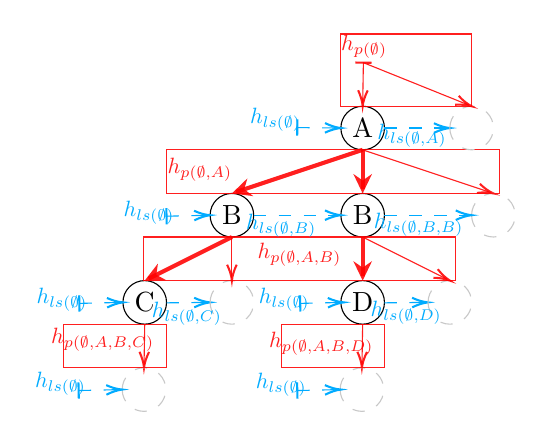
\begin{tikzpicture}[scale=0.7,x=0.75pt,y=0.75pt,yscale=-1,xscale=1]
		%uncomment if require: \path (0,336.6875); %set diagram left start at 0, and has height of 336.6875

		%Shape: Circle [id:dp5747539528933221] 
		\draw   (240,75) .. controls (240,66.72) and (246.72,60) .. (255,60) .. controls (263.28,60) and (270,66.72) .. (270,75) .. controls (270,83.28) and (263.28,90) .. (255,90) .. controls (246.72,90) and (240,83.28) .. (240,75) -- cycle ;
		%Shape: Circle [id:dp6584741963271383] 
		\draw   (150,135) .. controls (150,126.72) and (156.72,120) .. (165,120) .. controls (173.28,120) and (180,126.72) .. (180,135) .. controls (180,143.28) and (173.28,150) .. (165,150) .. controls (156.72,150) and (150,143.28) .. (150,135) -- cycle ;
		%Shape: Circle [id:dp42608384351679063] 
		\draw   (240,135) .. controls (240,126.72) and (246.72,120) .. (255,120) .. controls (263.28,120) and (270,126.72) .. (270,135) .. controls (270,143.28) and (263.28,150) .. (255,150) .. controls (246.72,150) and (240,143.28) .. (240,135) -- cycle ;
		%Shape: Circle [id:dp4039562507165959] 
		\draw   (90,195) .. controls (90,186.72) and (96.72,180) .. (105,180) .. controls (113.28,180) and (120,186.72) .. (120,195) .. controls (120,203.28) and (113.28,210) .. (105,210) .. controls (96.72,210) and (90,203.28) .. (90,195) -- cycle ;
		%Shape: Circle [id:dp6061665496522999] 
		\draw   (240,195) .. controls (240,186.72) and (246.72,180) .. (255,180) .. controls (263.28,180) and (270,186.72) .. (270,195) .. controls (270,203.28) and (263.28,210) .. (255,210) .. controls (246.72,210) and (240,203.28) .. (240,195) -- cycle ;
		%Straight Lines [id:da5328040663765743] 
		\draw [color={rgb, 255:red, 255; green, 0; blue, 0 }  ,draw opacity=0.88 ][line width=1.5]    (255,90) -- (167.85,119.05) ;
		\draw [shift={(165,120)}, rotate = 341.57] [fill={rgb, 255:red, 255; green, 0; blue, 0 }  ,fill opacity=0.88 ][line width=1.5]  [draw opacity=0] (13.4,-6.43) -- (0,0) -- (13.4,6.44) -- (8.9,0) -- cycle    ;

		%Straight Lines [id:da567244828908992] 
		\draw [color={rgb, 255:red, 255; green, 0; blue, 0 }  ,draw opacity=0.88 ][line width=1.5]    (255,90) -- (255,117) ;
		\draw [shift={(255,120)}, rotate = 270] [fill={rgb, 255:red, 255; green, 0; blue, 0 }  ,fill opacity=0.88 ][line width=1.5]  [draw opacity=0] (13.4,-6.43) -- (0,0) -- (13.4,6.44) -- (8.9,0) -- cycle    ;

		%Straight Lines [id:da20403721062923252] 
		\draw [color={rgb, 255:red, 255; green, 0; blue, 0 }  ,draw opacity=0.88 ][line width=1.5]    (165,150) -- (107.68,178.66) ;
		\draw [shift={(105,180)}, rotate = 333.43] [fill={rgb, 255:red, 255; green, 0; blue, 0 }  ,fill opacity=0.88 ][line width=1.5]  [draw opacity=0] (13.4,-6.43) -- (0,0) -- (13.4,6.44) -- (8.9,0) -- cycle    ;

		%Straight Lines [id:da25420509470673447] 
		\draw [color={rgb, 255:red, 255; green, 0; blue, 0 }  ,draw opacity=0.88 ][line width=1.5]    (255,150) -- (255,177) ;
		\draw [shift={(255,180)}, rotate = 270] [fill={rgb, 255:red, 255; green, 0; blue, 0 }  ,fill opacity=0.88 ][line width=1.5]  [draw opacity=0] (13.4,-6.43) -- (0,0) -- (13.4,6.44) -- (8.9,0) -- cycle    ;

		%Straight Lines [id:da060062721758333826] 
		\draw [color={rgb, 255:red, 255; green, 0; blue, 0 }  ,draw opacity=0.88 ]   (105,210) -- (104.53,238) ;
		\draw [shift={(104.5,240)}, rotate = 270.95] [color={rgb, 255:red, 255; green, 0; blue, 0 }  ,draw opacity=0.88 ][line width=0.75]    (10.93,-3.29) .. controls (6.95,-1.4) and (3.31,-0.3) .. (0,0) .. controls (3.31,0.3) and (6.95,1.4) .. (10.93,3.29)   ;

		%Straight Lines [id:da9112525130551028] 
		\draw [color={rgb, 255:red, 255; green, 0; blue, 0 }  ,draw opacity=0.88 ]   (255,210) -- (254.53,238) ;
		\draw [shift={(254.5,240)}, rotate = 270.95] [color={rgb, 255:red, 255; green, 0; blue, 0 }  ,draw opacity=0.88 ][line width=0.75]    (10.93,-3.29) .. controls (6.95,-1.4) and (3.31,-0.3) .. (0,0) .. controls (3.31,0.3) and (6.95,1.4) .. (10.93,3.29)   ;

		%Straight Lines [id:da42382449393367416] 
		\draw [color={rgb, 255:red, 255; green, 0; blue, 0 }  ,draw opacity=0.88 ]   (255,90) -- (343.1,119.37) ;
		\draw [shift={(345,120)}, rotate = 198.43] [color={rgb, 255:red, 255; green, 0; blue, 0 }  ,draw opacity=0.88 ][line width=0.75]    (10.93,-3.29) .. controls (6.95,-1.4) and (3.31,-0.3) .. (0,0) .. controls (3.31,0.3) and (6.95,1.4) .. (10.93,3.29)   ;

		%Shape: Circle [id:dp9771338101075551] 
		\draw  [color={rgb, 255:red, 200; green, 200; blue, 200 }  ,draw opacity=1 ][dash pattern={on 4.5pt off 4.5pt}] (330,135) .. controls (330,126.72) and (336.72,120) .. (345,120) .. controls (353.28,120) and (360,126.72) .. (360,135) .. controls (360,143.28) and (353.28,150) .. (345,150) .. controls (336.72,150) and (330,143.28) .. (330,135) -- cycle ;
		%Straight Lines [id:da75928763497055] 
		\draw [color={rgb, 255:red, 0; green, 171; blue, 255 }  ,draw opacity=1 ] [dash pattern={on 4.5pt off 4.5pt}]  (180,135) -- (238,135) ;
		\draw [shift={(240,135)}, rotate = 180] [color={rgb, 255:red, 0; green, 171; blue, 255 }  ,draw opacity=1 ][line width=0.75]    (10.93,-3.29) .. controls (6.95,-1.4) and (3.31,-0.3) .. (0,0) .. controls (3.31,0.3) and (6.95,1.4) .. (10.93,3.29)   ;

		%Straight Lines [id:da8384243170280115] 
		\draw [color={rgb, 255:red, 0; green, 171; blue, 255 }  ,draw opacity=1 ] [dash pattern={on 4.5pt off 4.5pt}]  (120,195.31) -- (148,195.02) ;
		\draw [shift={(150,195)}, rotate = 539.4] [color={rgb, 255:red, 0; green, 171; blue, 255 }  ,draw opacity=1 ][line width=0.75]    (10.93,-3.29) .. controls (6.95,-1.4) and (3.31,-0.3) .. (0,0) .. controls (3.31,0.3) and (6.95,1.4) .. (10.93,3.29)   ;

		%Shape: Circle [id:dp852651930656483] 
		\draw  [color={rgb, 255:red, 200; green, 200; blue, 200 }  ,draw opacity=1 ][dash pattern={on 4.5pt off 4.5pt}] (150,195) .. controls (150,186.72) and (156.72,180) .. (165,180) .. controls (173.28,180) and (180,186.72) .. (180,195) .. controls (180,203.28) and (173.28,210) .. (165,210) .. controls (156.72,210) and (150,203.28) .. (150,195) -- cycle ;
		%Straight Lines [id:da33797387516994126] 
		\draw [color={rgb, 255:red, 255; green, 0; blue, 0 }  ,draw opacity=0.88 ]   (165,150) -- (165,178) ;
		\draw [shift={(165,180)}, rotate = 270] [color={rgb, 255:red, 255; green, 0; blue, 0 }  ,draw opacity=0.88 ][line width=0.75]    (10.93,-3.29) .. controls (6.95,-1.4) and (3.31,-0.3) .. (0,0) .. controls (3.31,0.3) and (6.95,1.4) .. (10.93,3.29)   ;

		%Shape: Circle [id:dp7781216259767076] 
		\draw  [color={rgb, 255:red, 200; green, 200; blue, 200 }  ,draw opacity=1 ][dash pattern={on 4.5pt off 4.5pt}] (89.5,255) .. controls (89.5,246.72) and (96.22,240) .. (104.5,240) .. controls (112.78,240) and (119.5,246.72) .. (119.5,255) .. controls (119.5,263.28) and (112.78,270) .. (104.5,270) .. controls (96.22,270) and (89.5,263.28) .. (89.5,255) -- cycle ;
		%Straight Lines [id:da7533173940295115] 
		\draw [color={rgb, 255:red, 0; green, 171; blue, 255 }  ,draw opacity=1 ] [dash pattern={on 4.5pt off 4.5pt}]  (270,195.31) -- (298,195.02) ;
		\draw [shift={(300,195)}, rotate = 539.4] [color={rgb, 255:red, 0; green, 171; blue, 255 }  ,draw opacity=1 ][line width=0.75]    (10.93,-3.29) .. controls (6.95,-1.4) and (3.31,-0.3) .. (0,0) .. controls (3.31,0.3) and (6.95,1.4) .. (10.93,3.29)   ;

		%Shape: Circle [id:dp739418235900434] 
		\draw  [color={rgb, 255:red, 200; green, 200; blue, 200 }  ,draw opacity=1 ][dash pattern={on 4.5pt off 4.5pt}] (300,195) .. controls (300,186.72) and (306.72,180) .. (315,180) .. controls (323.28,180) and (330,186.72) .. (330,195) .. controls (330,203.28) and (323.28,210) .. (315,210) .. controls (306.72,210) and (300,203.28) .. (300,195) -- cycle ;
		%Straight Lines [id:da5061830263709963] 
		\draw [color={rgb, 255:red, 255; green, 0; blue, 0 }  ,draw opacity=0.88 ]   (255,150) -- (313.21,179.11) ;
		\draw [shift={(315,180)}, rotate = 206.57] [color={rgb, 255:red, 255; green, 0; blue, 0 }  ,draw opacity=0.88 ][line width=0.75]    (10.93,-3.29) .. controls (6.95,-1.4) and (3.31,-0.3) .. (0,0) .. controls (3.31,0.3) and (6.95,1.4) .. (10.93,3.29)   ;

		%Shape: Circle [id:dp4830940102467898] 
		\draw  [color={rgb, 255:red, 200; green, 200; blue, 200 }  ,draw opacity=1 ][dash pattern={on 4.5pt off 4.5pt}] (239.5,255) .. controls (239.5,246.72) and (246.22,240) .. (254.5,240) .. controls (262.78,240) and (269.5,246.72) .. (269.5,255) .. controls (269.5,263.28) and (262.78,270) .. (254.5,270) .. controls (246.22,270) and (239.5,263.28) .. (239.5,255) -- cycle ;
		%Straight Lines [id:da8687951733883794] 
		\draw [color={rgb, 255:red, 255; green, 0; blue, 0 }  ,draw opacity=0.88 ]   (255.5,30) -- (255.03,58) ;
		\draw [shift={(255,60)}, rotate = 270.95] [color={rgb, 255:red, 255; green, 0; blue, 0 }  ,draw opacity=0.88 ][line width=0.75]    (10.93,-3.29) .. controls (6.95,-1.4) and (3.31,-0.3) .. (0,0) .. controls (3.31,0.3) and (6.95,1.4) .. (10.93,3.29)   ;
		\draw [shift={(255.5,30)}, rotate = 270.95] [color={rgb, 255:red, 255; green, 0; blue, 0 }  ,draw opacity=0.88 ][line width=0.75]    (0,5.59) -- (0,-5.59)   ;
		%Straight Lines [id:da2320681357192822] 
		\draw [color={rgb, 255:red, 0; green, 171; blue, 255 }  ,draw opacity=1 ] [dash pattern={on 4.5pt off 4.5pt}]  (210,74.69) -- (238,74.98) ;
		\draw [shift={(240,75)}, rotate = 180.6] [color={rgb, 255:red, 0; green, 171; blue, 255 }  ,draw opacity=1 ][line width=0.75]    (10.93,-3.29) .. controls (6.95,-1.4) and (3.31,-0.3) .. (0,0) .. controls (3.31,0.3) and (6.95,1.4) .. (10.93,3.29)   ;
		\draw [shift={(210,74.69)}, rotate = 180.6] [color={rgb, 255:red, 0; green, 171; blue, 255 }  ,draw opacity=1 ][line width=0.75]    (0,5.59) -- (0,-5.59)   ;
		%Straight Lines [id:da9763574735032972] 
		\draw [color={rgb, 255:red, 0; green, 171; blue, 255 }  ,draw opacity=1 ] [dash pattern={on 4.5pt off 4.5pt}]  (60,195.69) -- (88,195.05) ;
		\draw [shift={(90,195)}, rotate = 538.69] [color={rgb, 255:red, 0; green, 171; blue, 255 }  ,draw opacity=1 ][line width=0.75]    (10.93,-3.29) .. controls (6.95,-1.4) and (3.31,-0.3) .. (0,0) .. controls (3.31,0.3) and (6.95,1.4) .. (10.93,3.29)   ;
		\draw [shift={(60,195.69)}, rotate = 538.69] [color={rgb, 255:red, 0; green, 171; blue, 255 }  ,draw opacity=1 ][line width=0.75]    (0,5.59) -- (0,-5.59)   ;
		%Straight Lines [id:da46410867028671343] 
		\draw [color={rgb, 255:red, 0; green, 171; blue, 255 }  ,draw opacity=1 ] [dash pattern={on 4.5pt off 4.5pt}]  (120,135.69) -- (148,135.05) ;
		\draw [shift={(150,135)}, rotate = 538.69] [color={rgb, 255:red, 0; green, 171; blue, 255 }  ,draw opacity=1 ][line width=0.75]    (10.93,-3.29) .. controls (6.95,-1.4) and (3.31,-0.3) .. (0,0) .. controls (3.31,0.3) and (6.95,1.4) .. (10.93,3.29)   ;
		\draw [shift={(120,135.69)}, rotate = 538.69] [color={rgb, 255:red, 0; green, 171; blue, 255 }  ,draw opacity=1 ][line width=0.75]    (0,5.59) -- (0,-5.59)   ;
		%Shape: Rectangle [id:dp9442762725540359] 
		\draw  [color={rgb, 255:red, 255; green, 0; blue, 0 }  ,draw opacity=0.88 ] (120,90) -- (349,90) -- (349,120) -- (120,120) -- cycle ;
		%Shape: Rectangle [id:dp46916019889141514] 
		\draw  [color={rgb, 255:red, 255; green, 0; blue, 0 }  ,draw opacity=0.88 ] (104,150) -- (319,150) -- (319,180) -- (104,180) -- cycle ;
		%Straight Lines [id:da250704382329064] 
		\draw [color={rgb, 255:red, 0; green, 171; blue, 255 }  ,draw opacity=1 ] [dash pattern={on 4.5pt off 4.5pt}]  (59.5,255.69) -- (87.5,255.05) ;
		\draw [shift={(89.5,255)}, rotate = 538.69] [color={rgb, 255:red, 0; green, 171; blue, 255 }  ,draw opacity=1 ][line width=0.75]    (10.93,-3.29) .. controls (6.95,-1.4) and (3.31,-0.3) .. (0,0) .. controls (3.31,0.3) and (6.95,1.4) .. (10.93,3.29)   ;
		\draw [shift={(59.5,255.69)}, rotate = 538.69] [color={rgb, 255:red, 0; green, 171; blue, 255 }  ,draw opacity=1 ][line width=0.75]    (0,5.59) -- (0,-5.59)   ;
		%Straight Lines [id:da7469552192135425] 
		\draw [color={rgb, 255:red, 0; green, 171; blue, 255 }  ,draw opacity=1 ] [dash pattern={on 4.5pt off 4.5pt}]  (210,255.69) -- (238,255.05) ;
		\draw [shift={(240,255)}, rotate = 538.69] [color={rgb, 255:red, 0; green, 171; blue, 255 }  ,draw opacity=1 ][line width=0.75]    (10.93,-3.29) .. controls (6.95,-1.4) and (3.31,-0.3) .. (0,0) .. controls (3.31,0.3) and (6.95,1.4) .. (10.93,3.29)   ;
		\draw [shift={(210,255.69)}, rotate = 538.69] [color={rgb, 255:red, 0; green, 171; blue, 255 }  ,draw opacity=1 ][line width=0.75]    (0,5.59) -- (0,-5.59)   ;
		%Straight Lines [id:da577886155294407] 
		\draw [color={rgb, 255:red, 0; green, 171; blue, 255 }  ,draw opacity=1 ] [dash pattern={on 4.5pt off 4.5pt}]  (212,195.69) -- (240,195.05) ;
		\draw [shift={(242,195)}, rotate = 538.69] [color={rgb, 255:red, 0; green, 171; blue, 255 }  ,draw opacity=1 ][line width=0.75]    (10.93,-3.29) .. controls (6.95,-1.4) and (3.31,-0.3) .. (0,0) .. controls (3.31,0.3) and (6.95,1.4) .. (10.93,3.29)   ;
		\draw [shift={(212,195.69)}, rotate = 538.69] [color={rgb, 255:red, 0; green, 171; blue, 255 }  ,draw opacity=1 ][line width=0.75]    (0,5.59) -- (0,-5.59)   ;
		%Straight Lines [id:da7835054268870489] 
		\draw [color={rgb, 255:red, 0; green, 171; blue, 255 }  ,draw opacity=1 ] [dash pattern={on 4.5pt off 4.5pt}]  (270,135) -- (328,135) ;
		\draw [shift={(330,135)}, rotate = 180] [color={rgb, 255:red, 0; green, 171; blue, 255 }  ,draw opacity=1 ][line width=0.75]    (10.93,-3.29) .. controls (6.95,-1.4) and (3.31,-0.3) .. (0,0) .. controls (3.31,0.3) and (6.95,1.4) .. (10.93,3.29)   ;

		%Straight Lines [id:da8246021494117906] 
		\draw [color={rgb, 255:red, 0; green, 171; blue, 255 }  ,draw opacity=1 ] [dash pattern={on 4.5pt off 4.5pt}]  (270,75) -- (313,75) ;
		\draw [shift={(315,75)}, rotate = 180] [color={rgb, 255:red, 0; green, 171; blue, 255 }  ,draw opacity=1 ][line width=0.75]    (10.93,-3.29) .. controls (6.95,-1.4) and (3.31,-0.3) .. (0,0) .. controls (3.31,0.3) and (6.95,1.4) .. (10.93,3.29)   ;

		%Shape: Circle [id:dp14086195915841282] 
		\draw  [color={rgb, 255:red, 200; green, 200; blue, 200 }  ,draw opacity=1 ][dash pattern={on 4.5pt off 4.5pt}] (315,75) .. controls (315,66.72) and (321.72,60) .. (330,60) .. controls (338.28,60) and (345,66.72) .. (345,75) .. controls (345,83.28) and (338.28,90) .. (330,90) .. controls (321.72,90) and (315,83.28) .. (315,75) -- cycle ;
		%Straight Lines [id:da5272161259387991] 
		\draw [color={rgb, 255:red, 255; green, 0; blue, 0 }  ,draw opacity=0.88 ]   (255.5,30) -- (328.14,59.25) ;
		\draw [shift={(330,60)}, rotate = 201.93] [color={rgb, 255:red, 255; green, 0; blue, 0 }  ,draw opacity=0.88 ][line width=0.75]    (10.93,-3.29) .. controls (6.95,-1.4) and (3.31,-0.3) .. (0,0) .. controls (3.31,0.3) and (6.95,1.4) .. (10.93,3.29)   ;

		%Shape: Rectangle [id:dp7842787512852565] 
		\draw  [color={rgb, 255:red, 255; green, 0; blue, 0 }  ,draw opacity=0.88 ] (240,10.31) -- (330,10.31) -- (330,60) -- (240,60) -- cycle ;
		%Shape: Rectangle [id:dp6269636709503503] 
		\draw  [color={rgb, 255:red, 255; green, 0; blue, 0 }  ,draw opacity=0.88 ] (49,210) -- (120,210) -- (120,240) -- (49,240) -- cycle ;
		%Shape: Rectangle [id:dp035044351208313174] 
		\draw  [color={rgb, 255:red, 255; green, 0; blue, 0 }  ,draw opacity=0.88 ] (199,210) -- (270,210) -- (270,240) -- (199,240) -- cycle ;

		% Text Node
		\draw (255,75) node  [align=left] {A};
		% Text Node
		\draw (165,135) node  [align=left] {B};
		% Text Node
		\draw (255,195) node  [align=left] {D};
		% Text Node
		\draw (105,195) node  [align=left] {C};
		% Text Node
		\draw (255,135) node  [align=left] {B};
		% Text Node
		\draw (195,69.5) node [scale=0.8,color={rgb, 255:red, 0; green, 171; blue, 255 }  ,opacity=1 ] [align=left] {$\displaystyle h_{ls( \emptyset )}$};
		% Text Node
		\draw (47,251) node [scale=0.8,color={rgb, 255:red, 0; green, 171; blue, 255 }  ,opacity=1 ] [align=left] {$\displaystyle h_{ls( \emptyset )}$};
		% Text Node
		\draw (143,103.5) node [scale=0.8,color={rgb, 255:red, 255; green, 0; blue, 0 }  ,opacity=0.88 ] [align=left] {$\displaystyle h_{p( \emptyset ,A)}$};
		% Text Node
		\draw (256,19) node [scale=0.8,color={rgb, 255:red, 255; green, 0; blue, 0 }  ,opacity=0.88 ] [align=left] {$\displaystyle h_{p( \emptyset )}$};
		% Text Node
		\draw (211.5,162) node [scale=0.8,color={rgb, 255:red, 255; green, 0; blue, 0 }  ,opacity=0.88 ] [align=left] {$\displaystyle h_{p( \emptyset ,A,B)}$};
		% Text Node
		\draw (76,221) node [scale=0.8,color={rgb, 255:red, 255; green, 0; blue, 0 }  ,opacity=0.88 ] [align=left] {$\displaystyle h_{p( \emptyset ,A,B,C)}$};
		% Text Node
		\draw (48,193.5) node [scale=0.8,color={rgb, 255:red, 0; green, 171; blue, 255 }  ,opacity=1 ] [align=left] {$\displaystyle h_{ls( \emptyset )}$};
		% Text Node
		\draw (108,133) node [scale=0.8,color={rgb, 255:red, 0; green, 171; blue, 255 }  ,opacity=1 ] [align=left] {$\displaystyle h_{ls( \emptyset )}$};
		% Text Node
		\draw (134,203) node [scale=0.8,color={rgb, 255:red, 0; green, 171; blue, 255 }  ,opacity=1 ] [align=left] {$\displaystyle h_{ls( \emptyset ,C)}$};
		% Text Node
		\draw (226.5,223.5) node [scale=0.8,color={rgb, 255:red, 255; green, 0; blue, 0 }  ,opacity=0.88 ] [align=left] {$\displaystyle h_{p( \emptyset ,A,B,D)}$};
		% Text Node
		\draw (199,252) node [scale=0.8,color={rgb, 255:red, 0; green, 171; blue, 255 }  ,opacity=1 ] [align=left] {$\displaystyle h_{ls( \emptyset )}$};
		% Text Node
		\draw (201,193) node [scale=0.8,color={rgb, 255:red, 0; green, 171; blue, 255 }  ,opacity=1 ] [align=left] {$\displaystyle h_{ls( \emptyset )}$};
		% Text Node
		\draw (285,202) node [scale=0.8,color={rgb, 255:red, 0; green, 171; blue, 255 }  ,opacity=1 ] [align=left] {$\displaystyle h_{ls( \emptyset ,D)}$};
		% Text Node
		\draw (293.5,141.5) node [scale=0.8,color={rgb, 255:red, 0; green, 171; blue, 255 }  ,opacity=1 ] [align=left] {$\displaystyle h_{ls( \emptyset ,B,B)}$};
		% Text Node
		\draw (120,138) node  [align=left] {$ $};
		% Text Node
		\draw (199,142) node [scale=0.8,color={rgb, 255:red, 0; green, 171; blue, 255 }  ,opacity=1 ] [align=left] {$\displaystyle h_{ls( \emptyset ,B)}$};
		% Text Node
		\draw (289,80.5) node [scale=0.8,color={rgb, 255:red, 0; green, 171; blue, 255 }  ,opacity=1 ] [align=left] {$\displaystyle h_{ls( \emptyset ,A)}$};


		\end{tikzpicture}
		\caption{A subfigure}\label{fig:broken_2}
	\end{subfigure}
	\caption{Broken Example}\label{fig:broken}
\end{figure}


Doubly-recurrennt neural networks (DRNNs) are a direct application of relational 
decomposition, decoding a node with relations corresponding to ``parent'' and 
``left sibling'' (see \figref{fig:broken}). As seen here, DRNNs introduce the 
notion of direct topology prediction. Though this is implemented in our 
framework, we note that it is distinct from relational decomposition, andspecial 
end-of-sequence tokens can also be used to predict topology.

Unfortunately, as presented, DRNNs are insufficient for decoding ASTs. Because 
of the indepedence of the two decoding directions, all subtrees with the same 
root label must be identical. It is impossible to decode a program with, say, 
two differing variable assignment statements in a row, or two functions that 
don't have identical bodies.
%Put another way, a DRNN cannot discriminate between two programs that differ in 
%such ways.

%There is a fundametal issue. For example, in the context of program repair, if 
%B represents the head of an If.

% TODO: find paper name
% https://arxiv.org/pdf/1809.01854.pdf
Paper XYZ tries to fix this by adding in a reference to the parent. But that 
ultimately just pushes the problem farther down the line: nodes with the same 
no-sibling parent and same grandparent have to produce identical subtrees.

We propose two fixes. First, we can add in some form of linearization of the 
AST, as in Figure %TODO.

However, a linearization suffers from the fact that the relation effectively has 
little structure to work with and must learn over long distances.


Our second fix is seen in Figure %TODO.
Here, we are defining a \textit{functional relation}. In particular, we are 
extracting the subtree state from the most recently completed subtree. This 
requires the (reflexive) transitive closure of the parent relation, composed 
with the left sibling relation, (with two separate RNNNs).  The subtree state 
represents a summary

%subtree(reflexive_transitive_closure

To do so, we introduce another relational operator: functional dependence.


% \subsection{Decoding fixes}
% Linearization:
% For example, either the in-order or pre-order traversals.

% Collateral Lineage: Use TreeLSTM to generate a summary of the left sibling 
% subtree. Pass that summary to the left node.

% Link global state changes / variable usages?
% Actually easier: most nodes have a well-defined number of children, basically 
% the only leaves are Constants and IDs, can actually run executions. Well-defined 
% ASTs (as opposed to parse trees). Inject semantic information. Decomposable.  
% Scope. Compositionality.

%Caveats: variables, Compound, Expression List, Constants

% ......................................................................... }}}1

%\subsection{Bottom-Up Decoding}
%% ......................................................................... {{{1
%%See the appendix for a brief explanation.

%Bottom-up TreeLSTM generation: use hidden state to predict node, number of 

%We implemented it, but the task is rather limited given . Just as a proof of 
%concept, we even use TreeLSTM for nodes that have literally just one child or no 
%recurrence. That said, we have not found a task on which this is actually 
%useful. 

%siblings, and whether this fills a hole for a prior part of the tree?  Why is 
%this useful? Debugging example.
%% ......................................................................... }}}1

\subsection{Relative attention}
% .................................... {{{1

\newcommand{\Align}[1]{\mathrm{align}{\parens{#1}}}
\newcommand{\score}[1]{\mathrm{score}{\parens{#1}}}

Our usual notion of attention uses $h^\star$. However, we can instead attend to 
the individual $h^r$. Generalizing one particular encantation of attention, we 
have:
%For a given step $t$ in decoding, we have (the softmax is over $i$, from $1$ to 
%$n$).
% \begin{align*}
% 	\score{s_{t-1}, \vh^r_i} &= 
% 	\parens{\rvv_a^r}^\top\tanh{\parens{\rmW^r_a[s_{t-1};\vh^r_i]}}\\
% 	\Align{y_t,x_i, r} &= \score{s_{t-1},\vh^r_i} \\
% 	\alpha^r_{t,i} &= \softmax{\parens{\Align{y_t, x_i, r}}} \\
% 	c^r_{t} &= \sum_{i=1}^n\alpha^r_{t,i}\vh^r_i \\
% 	c^\star_t &= \phi{\parens{%
% 		\sum_{\er \in \relations}\left.
% 			\rmU_a^r \vh^r_i
% 		\right.
% 	}}
% \end{align*}

%Once again, we choose $\phi=\tanh$.
\begin{align*}
	\mQ^r &= \rmW_Q^r \times \mX_Q^r \\
	\mK^r &= \rmW_K^r \times \mX_K^r \\
	\mV^r &= \rmW_V^r \times \mX_V^r \\
	\mZ^r &= \softmax{\parens{\frac{\mQ^r \times 
\parens{\mK^r}^\top}{\sqrt{d_k}}}}\mV^r \\
	\mZ^\star_t &= \phi{\parens{%
		\sum_{\er \in \relations}\left.
			\rmU_a^r \mZ^r
	\right.}}
\end{align*}

In practice, we used $\phi=\tanh$.  Aside from the last line, if we ignore the 
relational superscript and set $\mX_Q=\mX_K=\mX_V=\mX$, this is identical to the 
self-attention used in Transformer. The last line then aggregates the individual 
relative attentions for the final context.

Intuitively, by separating the attention components, relative attention provides 
greater flexibility in alignment within a graph. For example, in a tree with 
parent and left-sibling relations, we can independently evaluate the height and 
width alignment.


% TODO: cite
%The extension to relative self-attention is straightforward. Rather than pack 
%our embeddings $h^\star$ into $\mX$, we instead pack each individual $h^r$, We 
%could furthermore modify $\mX$ to only contain elements from the path, but we 
%don't attempt that in this work.
%
%We then use $c_i$ in place of $h_i$ when decoding.
%
%% TODO: cite attnetionn
%Attention is just another way of re-encoding inputs, and can also be decomposed.  
%Rather than calculate attention based on $h_i^\star$, we focus attention over 
%the individual relative hidden states, and combine the relative attentions to 
%obtain a final weight for the given hidden state. Alternatively, we could use 
%this combination of relative attentions directly, not needing to refer back to 
%the hidden state (is this like Transformer?), but we haven't implemented that.
%
%We can also attend to only a subset of the 
%
%The weights themselves can vary based on the current position of the node?
%
%This generalizes both attention and self-attention.

% TODO: relative attention, since decomposed attention is already taken.

Taking this one step further, we apply relative attention to pointer networks.
Pointer networks
%TODO \cite
work around a limited NN vocabulary by using the highest-weighted input as the 
output of the current step. For example, in generating an abstract syntax tree, 
rather than output ``arbitraryIdentifierName'' at some time step, the network 
can instead say ``output whatever the name of whatever variable was used over 
here at this place in the code''.

A relational pointer network can more directly encode the notion of where and 
how the variable was used, rather than the aggregate predictive state vector 
$\vh^\star$.

A few papers experimented with this method. XYZ used this method. ABC used it 
over linear.

% ID resolution can either be concurrent with tree generation or can take place 
% after. This gives the important distinction between decoding and encoding. If 
% after, the structure of the entire network is really the input to a new decoder, 
% for decoding IDs. However, this excludes the actual variable being used from 
% future decoding steps.

% Note that we could also use semantic / execution trace information, or even 
% combine the two!

% Lke the one paper, we can also feed in the attention context vector to the next 
% step of decoding. But wait, there's more! The attention context vector can 
% itself be treated as a relational decomposition, 

% Taking this one step further,

%Finally, when doing bottom-up encoding, this context can be used, too.
%TreeLSTM attention




% ......................................................................... }}}1

%\subsection{Library Implementation (Trooper)}
% ......................................................................... {{{1

%Creating fields from relations:
%In general, can fold over paths
%
%At graph level, we specify the functions
%At node level, we specify the inputs
%
%Encoder(sequence):
%% Automatically attach new RNN of appropriate shape/size, unless one is passed 
%% in with different parameters or something.
%% Create_path(converse(forward), reverse_rnn)
%Fold RNN f over forward path: encoding, parameterized input
%%Attach RNN r to reverse path
%
%Decoder(sequence):
%Attach RNN d to forward path with initial input tail(encoder(forward_path))
%prediction = map(pre["forward"], predict_label)
%if training:
%	loss = fold(error(label_prediction, actual_label), +)
%
%
%
%encoder = sequence() % has a "forward" path
%%encoder.converse("backwards") % can also specify sharing of weights
%
%% take initial state from final encoder forward state
%decoder = sequence(input=(encoder, "forward"))
%decoder.add_predictor("label", "forward")
%% alternatively, we don't need "last" if we have end-of-sequence token
%decoder.add_predictor("last", ["forward", "label"])
%
%encoder.feed(input_sequence)
%if training:
%	decoder.feed(output_sequence)
%	loss = decoder.reduce(label_loss)
%	loss += decoder.reduce(last_loss)
%else:
%	% this is where we'd implement beam search
%	decoder.next = lambda node: \
%		argmax(node.predictors["label"]) \
%			if node.predictors["last"] < 0.5 else
%		None
%
%	decoder.get_sequence()
%
%%In fact, these are all built in! Passing ``feed'' overrides the notion of 
%	%"next", so really this could also be written:
%
%% map stores the result in the node
%%encoder.map("combined", lambda node: concat(node["forward"], node["reverse"]))
%
%% one way of writing this! Keeps it modular. Basically, doesn't require a back 
%% arrow into every single decode step
%decoder.map("context_vector", lambda node: attention(node.edges["input"], 
%node.edges["forward"]))
%
%Attention itself then takes the transitive closure of node.edges["input"]
%
%Self attention is even simpler:
%
%decoder.map("context_vector", lambda node: attention(node.edges["forward"]))
%
%encoder.converse("backwards")
%decoder = sequence(input=(encoder, ["forwards", "backwards"]))
%
%
%%encoder
%%attention = functional_relation(encoded_state, decoded_state)
%%attention.map("weights", softmax(align(encoded_state, decoded_state)))
%%attention.map("weights", softmax(align(encoded_state, decoded_state)))
%%context = attention.reduce(lambda node: node["weights"] & 
%%attention.encoder.transitive_closure("combined")
%%attention
%
%
%
%
%
%Node
%----
%Needs to have a function handle_encoder_forward and handle_encoder_reverse, 
%which returns the values that each should propagate forward. E.g., for encoding, 
%can just return the node's label
%
%For decoding, we might need to {\tt predict} that label
%handle_decoder_forward takes the form:
%	if label is None, predict
%else:
%	return label
%
%handle_decoder_predict
%
%Train:
%loss = map("label_prediction", label)
%reduce(loss, +)
%
%PNode:
%Feed loss(
%
%Train:
%Reduce(loss, +)

%Topological reasoning over order pairs of edge relations
%Topological reasoning as operations over paths of edge relations

%Forces mathematical reasoning about whether something makes sense.

%Relational thinking

%Two distinct parts: relational specifications, and functions over relations

%Simple set of building blocks for working with relations.
%Mapping vs folding an RNN over a tree

%In many cases, these are homogenous relations, especially if we only have one 
%node type

%Left-total, right-total

%Random paths?

%General relations: Can provide converse, composition, restrictions.
%map, reduce, apply

%Is the relation one to one, or one to many (N or ?), or many (N or ?) to one?

%Within specific structures, we can provide more, such as transitive closure if 
%we know that it is a partial order such as a sequence, tree, or DAG

%Provides composition, intersection, union, higher-order, concatenation, 
%converse, transitive closure

%Global reasoning vs local reasoning
%Base Case/inputs?

%inputs = Sequence
%outputs = Sequence
%connect(tail(inputs.next), head(outputs.next))


%% Separates training from specification of structure

%inputs = Sequence
%reverse = converse(inputs.next) # also a sequence
%context_vector = concat(tail(inputs.next), tail(reverse))# a vector
%connect(context_vector, head(outputs.next)) # optionally automatically transform 
%to correct size
%%connect(tail(inputs.next), head(outputs.next))
%%connect(tail(reverse), head(outputs.next)) # how to handle both?

%hpred = concat(inputs.next, reverse) # a sequence
%attention = transitive_closure(hpred)


%# Every operation is automatically parameterized unless told not to
%h = merge(hparent, hsibling)
%predict(h, label)
%predict(h + label, attr)
%predict(h + label + attr, topology)

%Predict
%-------
%hpred = something





%ForwardEncoder(Sequence)
%------------------------
%Forward is a Chain



%Classifier(Vector)
%------------------


%Predict
%-------
%Encoder.forward


%Decoder(Sequence)
%-----------------



%handleforward: Apply LSTM to <label, attr>

%1->2->3->4->5

%Node is a sequence, so:
%---
%Relations['Forward'][in/out]

%Label
%Attr




%Query for terminated paths?

%Sequence: Assumes a single ``next'' operator.
%Provides forward
%Backwards is then converse

%Tree: Assumes a single ``children'' operator.
%Within a tree, we assume relations form a partial order.
%Provides parent, left-sibling, left-inorder-predecessor, etc.

%Attention is a function over the transitive closure of a given relation.

%Validating the configuration of a model.



%% Comes closer to aligning the tensorflow computation graph with our visual 
%% intuition for what's going on.
%% 1) transform inputs (e.g., actual-word to one-hot, one-hot to word 
%% embeddings). The notion of a node in the tensorflow graph and in TROOPER are 
%% sometimes closely aligned. The right level of abstraction is somewhat 
%% task-specific. The transformation could be its own input type, or we'll leave 
%% transformations out of the Trooper graph.
%% 2)
%% 3) transform outputs (e.g., one-hot to actual word).

%Consider an implementation of a simple unidirectional Seq2Seq.

%We have edge types (see Figure XYZ). Transitive vs not transitive

%Mentally unroll the graph.

%(Input->Encoder)
%Encoder->Encoder
%Encoder->Decoder
%Decoder->Decoder
%(Decoder->Output)

%Encoder/Decoder are both:
%Sequence
%(Input->Internal)
%(Internal->Internal)
%(Internal->Output)

%Have no idea as to structure, aside from names of edges.

%Graph:
%Encoder
%Decoder

%Single datapoint
%Subgraph forward_inputs: Sequence(words)
%Subgraph reverse_inputs: Sequence(reverse(words))
%Subgraph forward_outputs: Sequence(translation)

%% TODO: sharing weights?

%Subgraph Encoder:
%% Takes in a graph with (at least) "forward" and "reverse" edges
%% Define functions over those edges, computing a new graph with those results
%% What is the ordering?
%Recurrence?
%Null start/end of encoding?
%forward_encoding = f(forward)
%reverse_encoding = r(reverse)

%Subgraph Decoder:
%output=[forward_encoding; reverse_encoding]
%Base case=Concatenate forward_encoding[-1], reverse_encoding[0]
%forward_decoding = g(output)


%% Takes in a graph with "encoded forward", "encoded reverse", and "forward" 
%% edges
%Create internal edge between first encoder state and first decoder state
%Create internal edge between last encoder state and first decoder state
%Compose relation(Concatenation those two)
%Create `forward' edge from that to first input
%Apply function d to forward


%Subgraph Predict:
%prediction = p(forward_decoding)
%% TOPOLOGY XXX ?
%% Takes in a graph with "decoded forward" edges.
%Apply function predict to p

%Subgraph Train:
%loss = e(prediction, output)
%Takes in/instantiates outputs and feeds them to decoder
%Apply loss function L to prediction_outcome
%total_loss = sum(loss)

%This isn't interesting, because we aren't doing anything particularly 
%higher-level with relations

%Optimize for matrix multiplication

%Can ignore what encoder is, since we just need edges from it

%DRNN
%----
%parent
%left_sibling


%DRNN+SeqC
%---------





%Create edge(encoder_context): encoder->internal relation
%															(vs encoder->node->internal relation)
%: RNN



%Encoder is a sequence
%Query for inputs
%Define input->encoding_node function
%Define encoding_node->encoding_node function




%How to connect subgraphs: query for info from other subgraph by relation?

%A ``node'' is just a convenient type of Subgraph, where edges and internal nodes 
%are implicit based on fields of the node.

%Subgraph needs to predict topology? Output of a node needs to be a set of new 
%nodes, and the old nodes relation to the node?

%Dynamic back-edge creation (queries). Everything within a subgraph automatically 
%gets propelled forward, but queries pull in inputs to do so.

%Query an internal node for some field, and base topology decision on that?


%Internal Node (subclass of subgraph):
%Fields vs topology



%End-of-sentence vs topology prediction.

%Relational Decomposition kernel vs helpers on top

%Some of these can be readily implemented as just wrappers around Tensorflow 
%operations/LSTMs/etc.


%Adding in bidirectionality:

%Within a subgraph:
%Attach a function to an edge type. An edge can use whatever's at the source node 
%as inputs.






%(A node can be seen as a subgraph, but in the implementation they are currently 
%distinct.)

%A node is a special case of a graph, where values can only depend on direct 
%inputs to the node.

%At any node, we automatically have access to all relation data pre and post, as 
%well as any inputs to our supergraph.

%Specify node fields, and if necessary, how to predict them.
%Back edges
%Forward edges


%My label is based on (leftsibling,parent)
%My topology is based on (leftsibling,parent,label)

%Config file

%Subgraph

%Takes advantage of the fact that tensorflow won't evaluate parts of the 
%computation graph that aren't actually used.
%Figuring out input edges of new node. As long as we specify the node type that 
%we're connecting to, that's easy. Forward edges vs back edges.

%Whether something is internal to a node or split across multiple nodes is a 
%matter of software engineering.

%Aggregation functions over multiple edge types: Sum, average, concatenate, 
%TreeLSTM, attention


%Provides a standardized way of explaining work.
%Readily visualize inputs, outputs, what's to be predicted, attention, etc..

%A subgraph works within the structure provided by the inputs/outputs

%A graph can create an edge between subgraphs?

%A subgraph takes inputs, which are the only thing that can be queried/create 
%edges?

%Decoder is itself a black box?
%Node type?

%h_pred = Relate(Encoder, Concatenate(forward, reverse))
%attention = Relate(Encoder, Attention(h_pred))

%1 result per terminated path/relation

%Decoder(Encoder.forward)
%vs
%Decoder(Attend(Encoder.forward))

%To define a graph G\@:
%List of names of subgraphs
%For each subgraph:
%	Identify RNN for each edge type. Results of edge types are stored at the 
%	source node.
%	1) Construct a query for the state from other nodes. For example, `` (this 
%	implicitly creates edges)
%	For each node hole, specify 1) the inputs, and 2) the function. We may want to 
%	predict the label before or after updating the RNN.
%	2) Topology prediction. The order of them matters.
%	(For now, everything is a DAG, so we never go back to an old node)


%	Combine my left sibling and my parent info to make a predictive vector about 
%	my state.

%	% Every node has a value, every edge has a type
%	% Do we only make predictions at nodes?

%	1) edge values
%	2) topology value?

%	Then, 

%	It's at the graph level that we specify what that means

%	For each edge type (identified by subgraph, relation name)

%		Specify what edge holes are possible? Labels are just edge types that point 
%		back to input dictionary. (Given this, pointer network become trivial)

%	How to train can automatically be inferred by the possible holes.

%Explicitly state which holes exist during training.

%Inheritance

%Many problems can be inversely transformed to such a form.


%Also makes it clear violations of data usage, etc.

%Define the subgraphs. Any node in the subgraph can be addressed by the label in 
%the subgraph.


%Inheritance

%Attend to all nodes





%Even just describing some sort of ``fold'' operation over your structure.

%Cleaner separation between structure and functionality.

%An easy way to specify decomposition. 

%Training, validation, and test stuff is outside the scope of the model, as are 
%hidden unit sizes, etc. Is that true?

%Focus on what really matters: too much time spent actually programming models, 
%spending 99\% of your time trying to get clean data.

%Training
%Validation
%Test

%Converting between models (invertible function to get back to the representation 
%output you want)

%Many models come down to just specifying an edge type.

%Groups of relations.

%Automatic topological sort.

%The flow of the graph constrains what we can and can't use.


%Need to define ordering over the graph.

%Edges from encoder nodes to decoder nodes are different edge types. Directly 
%work together without any extra effort.

%Inputs / Conditioned-on data
%----------------------------

%Graph
%-----
%Can be readily parallelized by embedding multiple disconnected graphs at the 
%same time.

%Inputs -> [Hole]

%Edge Hole
%----
%Local loss function?
%Here's how to predict what goes in a hole of this type.

%Decompositions
%--------------
%Generalizes equation XYZ

%$h^d$ is ultimately the concatenation of several decompositions of relations.

%Edge/Relation
%-------------
%What function does the relation represent?
%Transitive or nah?
%Higher-order relations
%% What operator do I use to validate the relation?
%What if there's a hole here? How to predict?


%Node-local view of info:
%------------------------
%How do fill in holes next to this node?

%If something can't be a hole, great!


%Need to predict local topology if decoding?
%In other words, output a set of ``does this edge exist''. Can either be to a 
%decoded node, or wondering if we have a right-sibling at all.
%Which node should be visited next?
%``If this is something I don't know, then do this to predict it''.

%How do we determine flow through the graph?

%A classifier just has an edge type from root to a single node vector 

%Furthermore, we can potentially handle multiple paths at once

%Enter node:
%Abstract syntax tree, we go as far as to use this to run a step in an 
%interpreter over the AST, short-circuit beam search,

%Influence direction of beam search, etc.

%Blurs the line between encoding and decoding. We now just have holes.

%Are we allowed to ask the question ``are we decoding?''.

%Leave node

%We predict label and attr separately. That is basically a second node hole.

%Limitations: does not currently batch well. We are literally iterating node by 
%node

%%This might vary by node type, as well. Specify node type as some boolean? Node 
%% types can be vectors of differing lengths,

%Can readily use scipy,numpy,tensorflow,etc.\ functionality in the implementation 
%of any of these things.

%``Connect two nodes if they have this in common''. We literally visit the tree.


%Need to define 

%(You can have multiple edges for the same relation if we want to capture 
%different functionality.)

%When training, we just have some nodes be holes 

%Connect to all nodes of type ``decoder'', or ``noun''
%I can be a left sibling.
%I can be a right sibling.
%I can be a parent.
%I can have a parent.
%What might I need to predict?
%Do I need to predict any local topology?

%Do I know my label? What is the task?

%Other nodes can inspect my state arbitrarily.

%Things like regularizing are outside the scope of a node.

%If What do I do under either of those scenarios?
%Differences between training time and test time?
%What if I attend to something for which I haven't yet decoded the output?
%Do I have to know whether I'm embedding or decoding?
%BERT (i.e., maskig)
%Predict my topology: am I the right-most sibling? What information can I use to 
%make that prediction?


%Limitations: Have not yet tried general graphs, non-backprop-able learning, etc.

%Ideally enables easier comparison with other models.

%DAG->Data

%Tree representations of object oriented programming edge relations.
%																				priors
%																										expert
%object oriented programmable edge relations

%Topological reasoning as object-oriented programmable edge relations

%Training representations of objects over edge relations
%Tensorflow
%Training relational 

%For any given input and output example, the user provides a list of vectors (in 
%matrix form), a list of edges (potentially including an edge type), and a 
%dictionary that maps edge types to: a function for the recurrence, properties of 
%the edge type (should it use attention, should it be transitive if not directly 
%specified, etc.)

%We also are in the process of implementing visualization over the attention.  
%Integrating convolution neural networks is an orthogonal task.

%Sensible defaults.

%Node-specific functions vs not-node-specific functions.

%Specifying encoding vs decoding vs end-to-end. The encoder or the decoder don't 
%have to be written in the library, but still trained end-to-end.

%Really, the ``kernel'' of the framework is tensorflow-specific, and otherwise 
%framework agnostic (though it is in Python).

%New functionality built into the library (such as attention using multiple 
%heads) is immediately applicable to any prior work.

%Currently, the library is a proof of concept, and as such things like batch 
%processing haven't been implemented. There is support for limited parallelism on 
%a single machine (such as parsing a tree), but no distributed. and 
%tensorboard/tensorflow debugging is limited.

%Pointer networks can similarly be encoded without even needing to touch the 
%kernel.


%Alternatively, given a DAG that extends from our own base class, we do also have 
%something that doesn't require the user needing to manually calculate the stuff.  
%The benefit of using the DAG is that one can immediately identify 

%For now, the construction of $\vh_i^\star$ is hard-coded, but we're expanding 
%that.

%Topology prediction is generalized to predicting either 1) if an edge should 
%exist between two nodes.

%We have a pre-defined list of 

%Furthermore, it warns about things like bidirectionality.

%% TODO: including dictionary translation or not

%Part of the implementation is defining 

%The decomposition framework also allows for easy programming.

%Currently limited to acyclic graphs for decoding.

%Additionally supports composition, higher-order, union,

%Readily works on sequential tasks.

%Paths are parallelizable

%Significant Engineering effort to production

% ......................................................................... }}}1

\section{Evaluation}\label{sec:evaluation}

\subsection{Methodology}

Python and Tensorflow Nvidia GeForce GTX 1080Ti

Cross-validation? Trained until convergence?

Each relation introduces $X$ new parameters. As such,
to keep the number of parameters across all tests roughly the same, 

%Analysis of emphasis of the components of hpred?

Compare against Seq2Tree, Tree2Seq, and Tree2Tree

\subsection{IFTTT Task}
Compare against the grammar paper and DRNN (and Seq2DRNN-SynC?).
For a fair comparison, we implemented the fix within the code of DRNN, available 
at. Note that this does not include.  IFTT

\subsection{Variable Hole Task}

Relational pointer networks. In this task, we But not misuse or name
Compared against the version where we just condition on $h_{pred}$, we get:

\subsection{NLP task\ldots}

\subsection{Program classification task / Program translation task}

\section{Conclusion}\label{sec:conclusionn}


\bibliography{iclr}
\bibliographystyle{style/iclr}

\appendix
\section{Appendix}

\end{document}
